\section{Introduction}
\label{sec:introduction}

Artificial life systems are a powerful technique for studying evolution and have yielded many important insights \citep{wilkeEvolutionDigitalOrganisms2001,zamanCoevolutionDrivesEmergence2014,goldsbyEvolutionaryOriginSomatic2014}.
Much of this power derives from the fact that these systems provide the ability to perfectly observe evolutionary dynamics.
In particular, research advances have often been made possible by analyzing phylogenetic data on the evolutionary trajectories that lead to a given outcome \citep{lenskiEvolutionaryOriginComplex2003,lalejiniEvolutionaryOriginsPhenotypic2016,johnsonEndosymbiosisBustInfluence2022a}.

While these analyses are powerful, phylogenetic data can quickly become large and unwieldy.
Thus, as artificial life systems and the questions we pose become more complex, better tools are needed.
These come in two forms: 1) evolutionary summary statistics that can be used to draw abstract insights from lineages and phylogenies \citep{dolsonInterpretingTapeLife2020}, and 2) algorithmic techniques for efficiently collecting phylogenetic data at scale \citep{morenoHereditaryStratigraphyGenome2022}.
Given that phylogenies are an abstraction that generalizes across all evolutionary contexts, they facilitate drawing conclusions that scale across different artificial life systems and biology.

%The utility of artificial life systems as an experimental platform to study evolution hinges on the ability to observe and interpret underlying evolutionary dynamics.
%As systems get more complex this problem gets more difficult.

%Phylogenetic analyses help with this problem by providing a window that generalizes across systems.
%These tools are commonly used to interpret evolutionary trajectories and stepping stones (Avida flame graphs, lalejini plasticity).
%This is important for understanding how evolutionary processes navigate the genetic search %space.
%Although less common, phylogenetic analyses have great potential to be used to characterize evolutionary dynamics such as selection pressure (i.e., ongoing adaptation) and ecological dynamics.
%These are of core interest to artificial life, particularly with respect to OEE.
Indeed, phylogeny-based metrics have already been used for varied purposes such as identifying hallmarks of open-ended evolution \citep{dolsonMODESToolboxMeasurements2019}, predicting which runs of evolutionary computation will be successful \citep{hernandezWhatCanPhylogenetic2022a,shahbandeganUntanglingPhylogeneticDiversity2022a}, quantifying patterns of tumor evolution \citep{scottInferringTumorProliferative2020,lewinsohnStatedependentEvolutionaryModels2023}, and identifying priorities for conservation \citep{forestPreservingEvolutionaryPotential2007}.
Much of the early work on quantifying phylogenetic properties has its origins in conservation biology and paleontology literature, as researchers in these fields attempted to draw inferences about the past from limited data.
More recently, medical researchers have embraced measuring phylogenies in real time in an effort to understand the evolution of pathogens and cancer.
% TODO: cite?

\begin{figure*}
  \begin{minipage}{1\columnwidth}
    \centering
    Generations Ago (approx.)
  \end{minipage}
  \hfill
  \begin{minipage}{1\columnwidth}
    \centering
    Generations Ago (approx.)
  \end{minipage}
  \begin{minipage}{1\columnwidth}
    \hspace{0.02\linewidth}
    \rotatebox{30}{\makebox[0.1\linewidth][c]{200,000}}
      \hfill
    \rotatebox{30}{\makebox[0.1\linewidth][c]{50,000}}
      \hfill
    \rotatebox{30}{\makebox[0.1\linewidth][c]{10,000}}
      \hfill
    \rotatebox{30}{\makebox[0.1\linewidth][c]{2,000}}
      \hfill
    \rotatebox{30}{\makebox[0.1\linewidth][c]{30}}
    \rotatebox{90}{\makebox[0.05\linewidth][c]{0}}
  \end{minipage}
  \hfill
  \begin{minipage}{1\columnwidth}
    \hspace{0.02\linewidth}
    \rotatebox{30}{\makebox[0.1\linewidth][c]{200,000}}
      \hfill
    \rotatebox{30}{\makebox[0.1\linewidth][c]{50,000}}
      \hfill
    \rotatebox{30}{\makebox[0.1\linewidth][c]{10,000}}
      \hfill
    \rotatebox{30}{\makebox[0.1\linewidth][c]{2,000}}
      \hfill
    \rotatebox{30}{\makebox[0.1\linewidth][c]{30}}
    \rotatebox{90}{\makebox[0.05\linewidth][c]{0}}
  \end{minipage}
  \begin{subfigure}[b]{1\columnwidth}
    % \begin{noindent}
    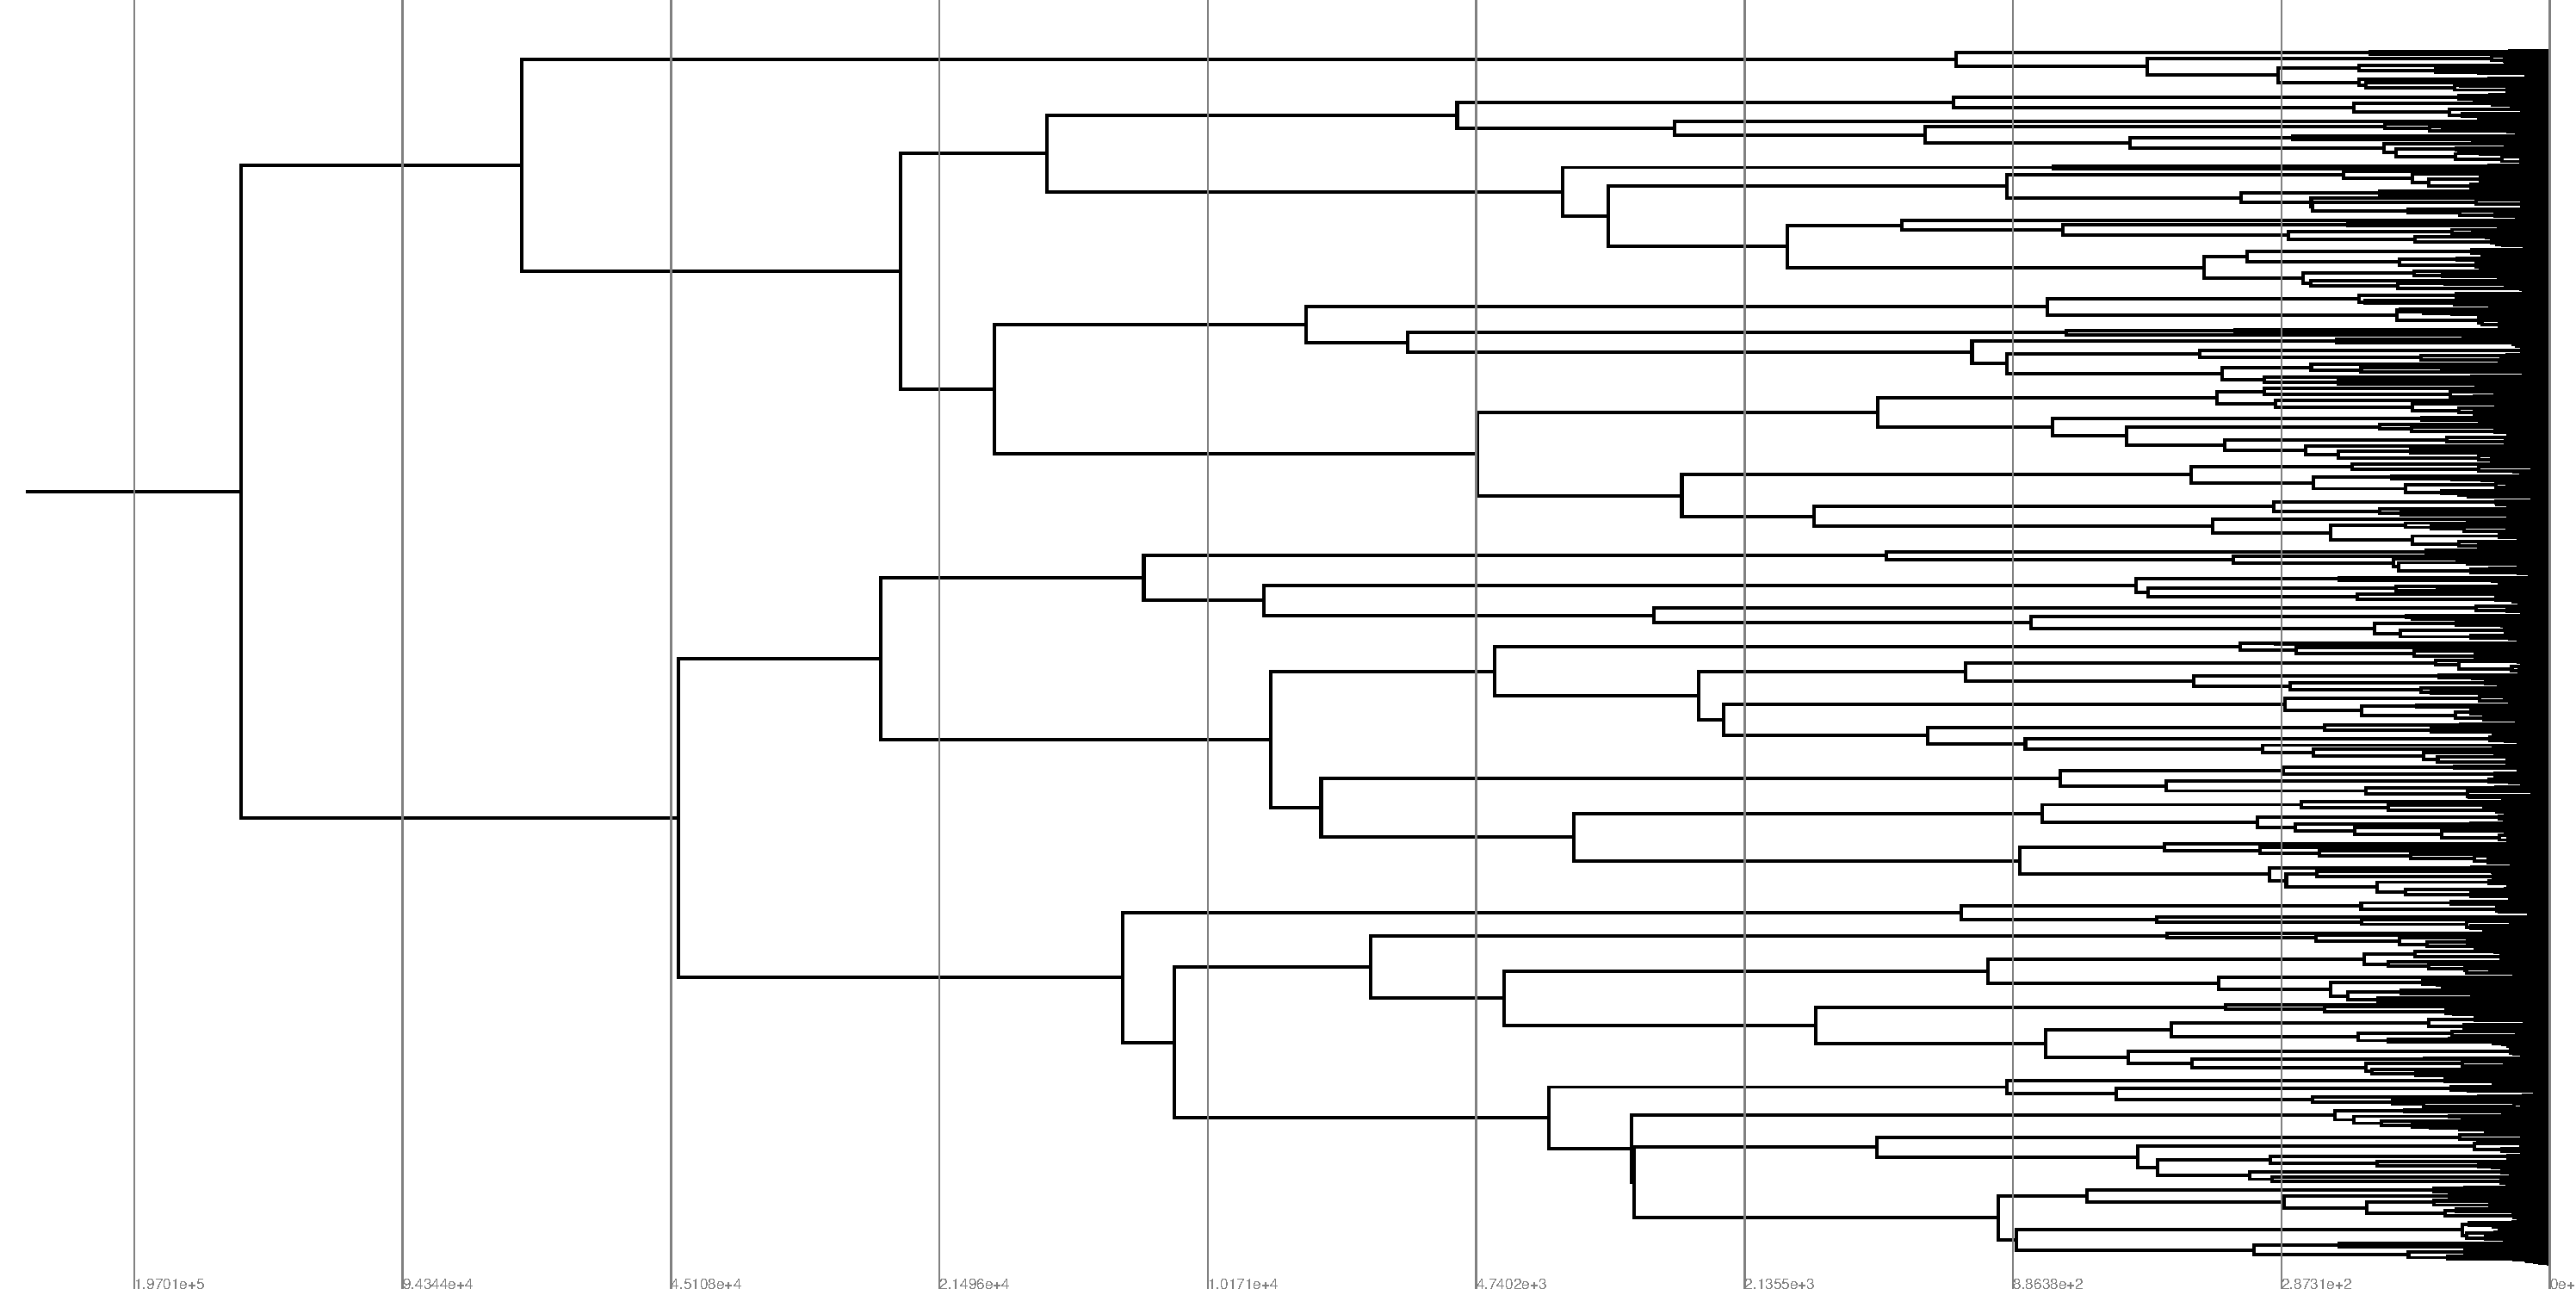
\includegraphics[height=0.12\textheight,width=\textwidth]{img/perfect-tree-phylogenies-log/epoch=7+resolution=3+treatment=0/a=collapsed-phylogeny+epoch=00007+mut_distn=np.random.standard_normal+num_generations=32768+num_islands=1024+num_niches=1+p_island_migration=0.01+p_niche_invasion=3.0517578125e-08+population_size=3276.../8+replicate=0+tournament_size=4+treatment=0+_generation=262144+_index=0+ext=.pdf}
    % \end{noindent}
    \caption{%
      spatial structure}
    % \label{fig:perfect-tree-phylogenies-log:TODO}
  \end{subfigure}
  \hfill
  \begin{subfigure}[b]{1\columnwidth}
    % \begin{noindent}
    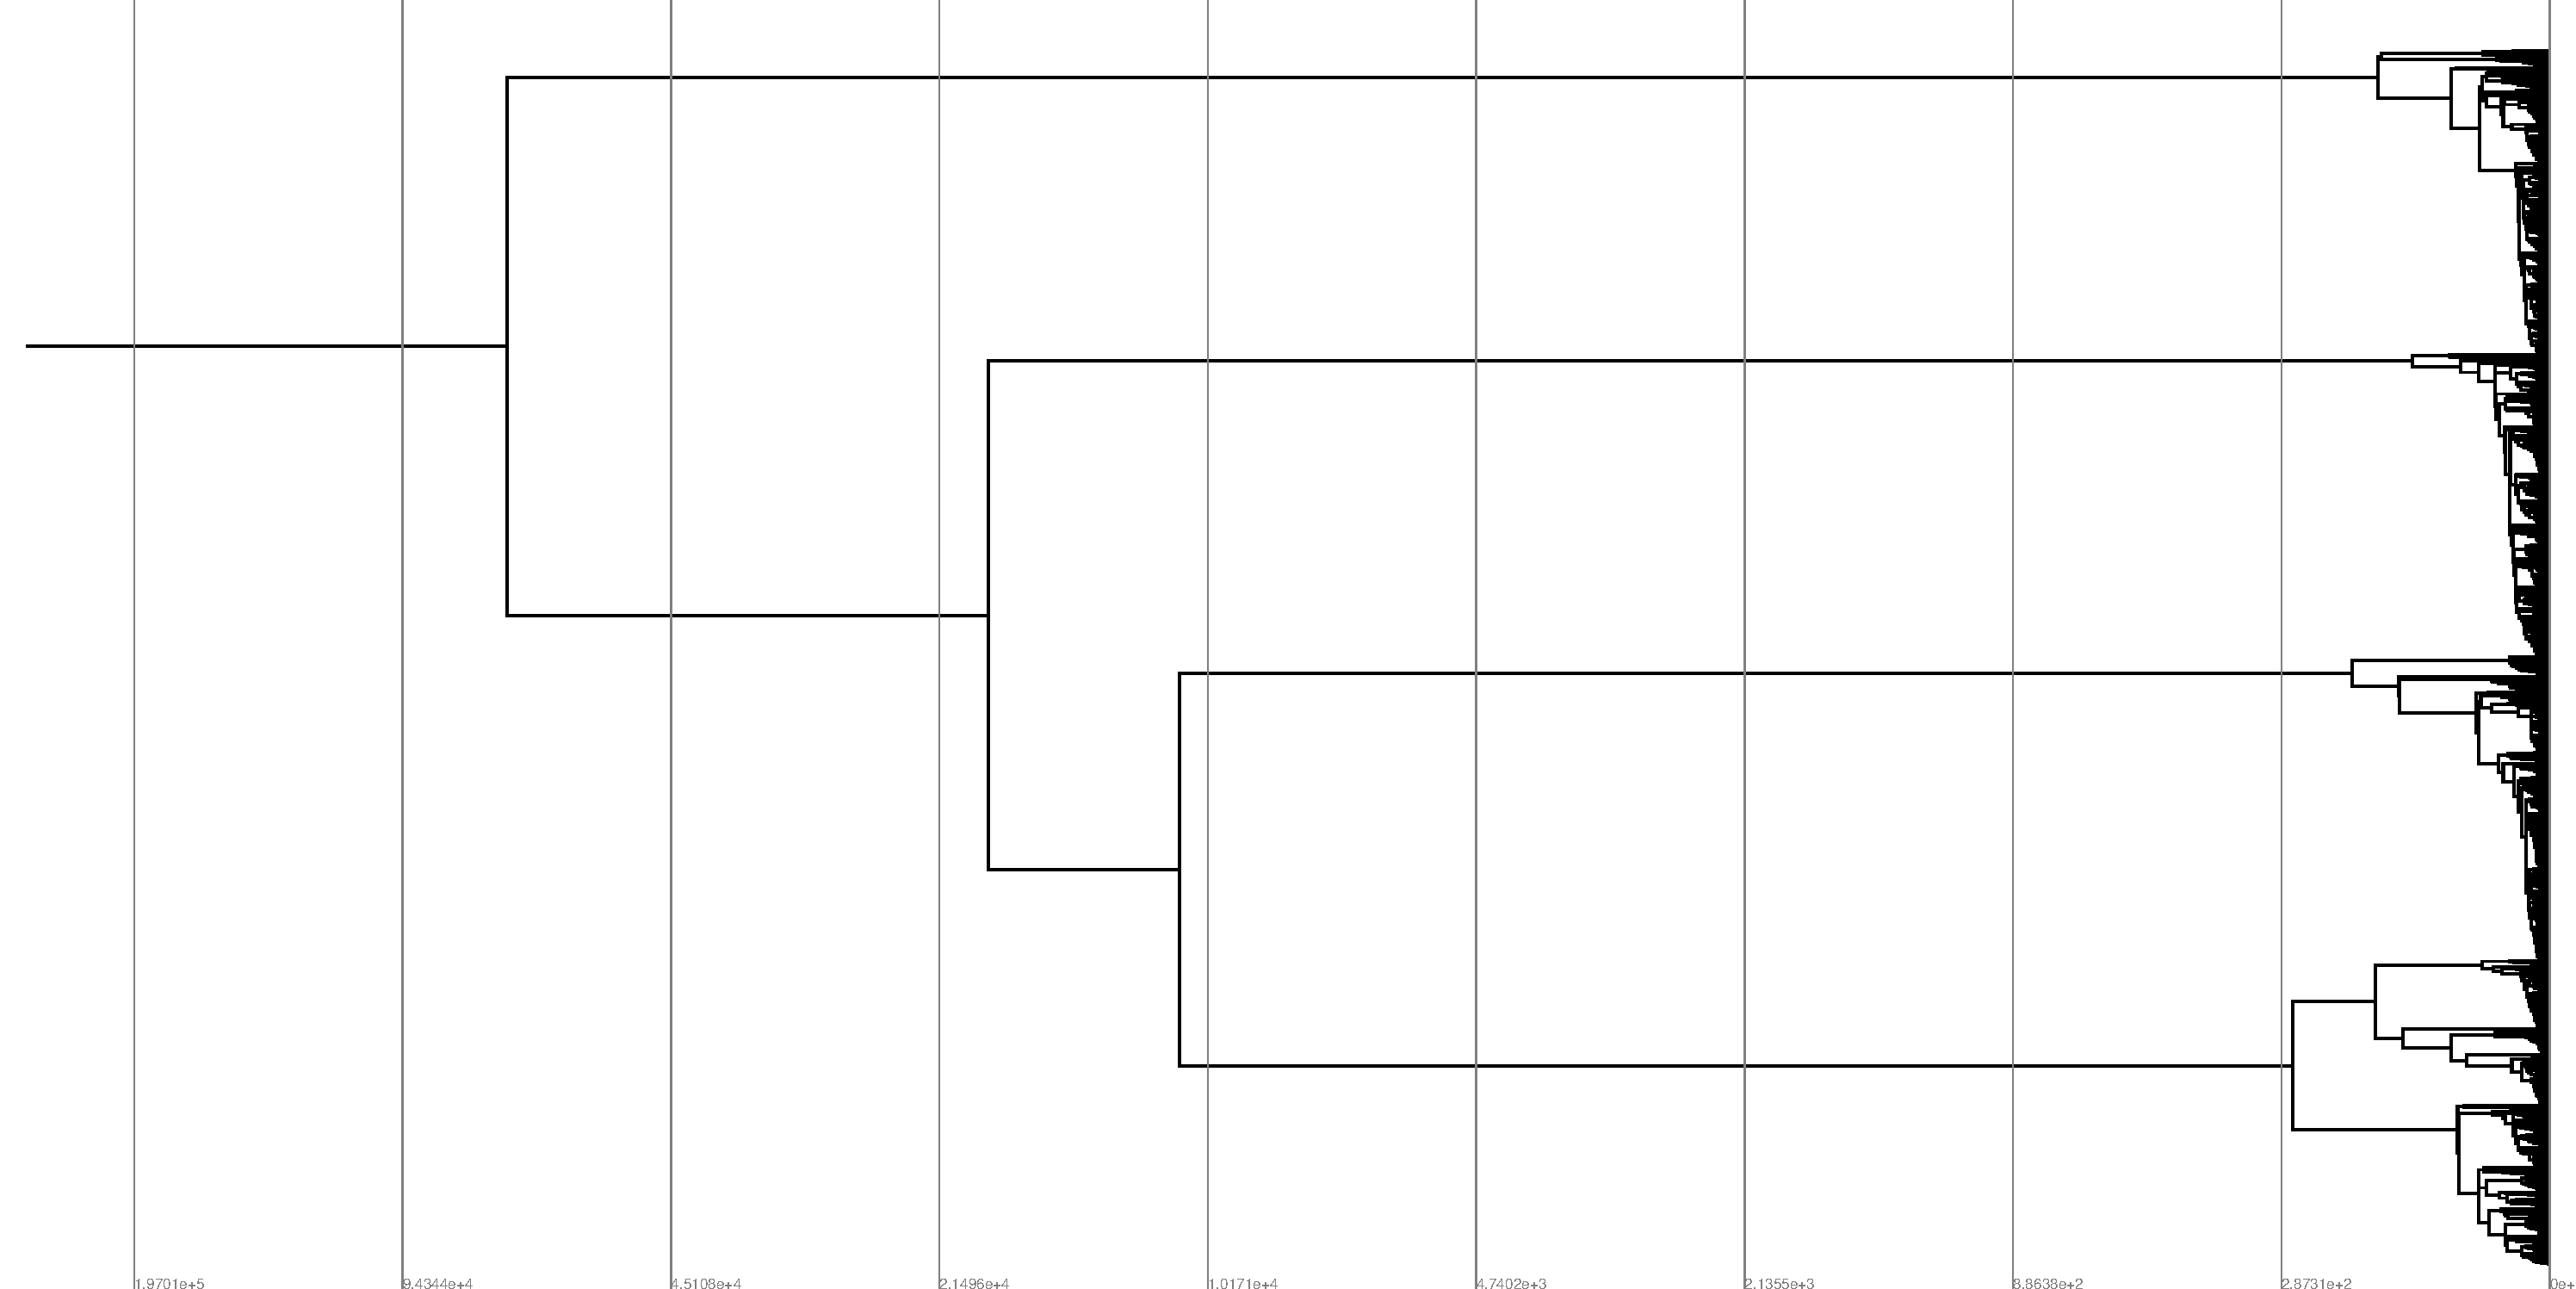
\includegraphics[height=0.12\textheight,width=\textwidth]{img/perfect-tree-phylogenies-log/epoch=7+resolution=3+treatment=10/a=collapsed-phylogeny+epoch=00007+mut_distn=np.random.standard_normal+num_generations=32768+num_islands=1+num_niches=4+p_island_migration=0.01+p_niche_invasion=3.0517578125e-08+population_size=32768+r.../eplicate=0+tournament_size=2+treatment=10+_generation=262144+_index=10+ext=.pdf}
    % \end{noindent}
    \caption{%
      4 niche ecology}
    % \label{fig:perfect-tree-phylogenies-log:TODO}
  \end{subfigure}
  \hfill
  \begin{subfigure}[b]{1\columnwidth}
    % \begin{noindent}
    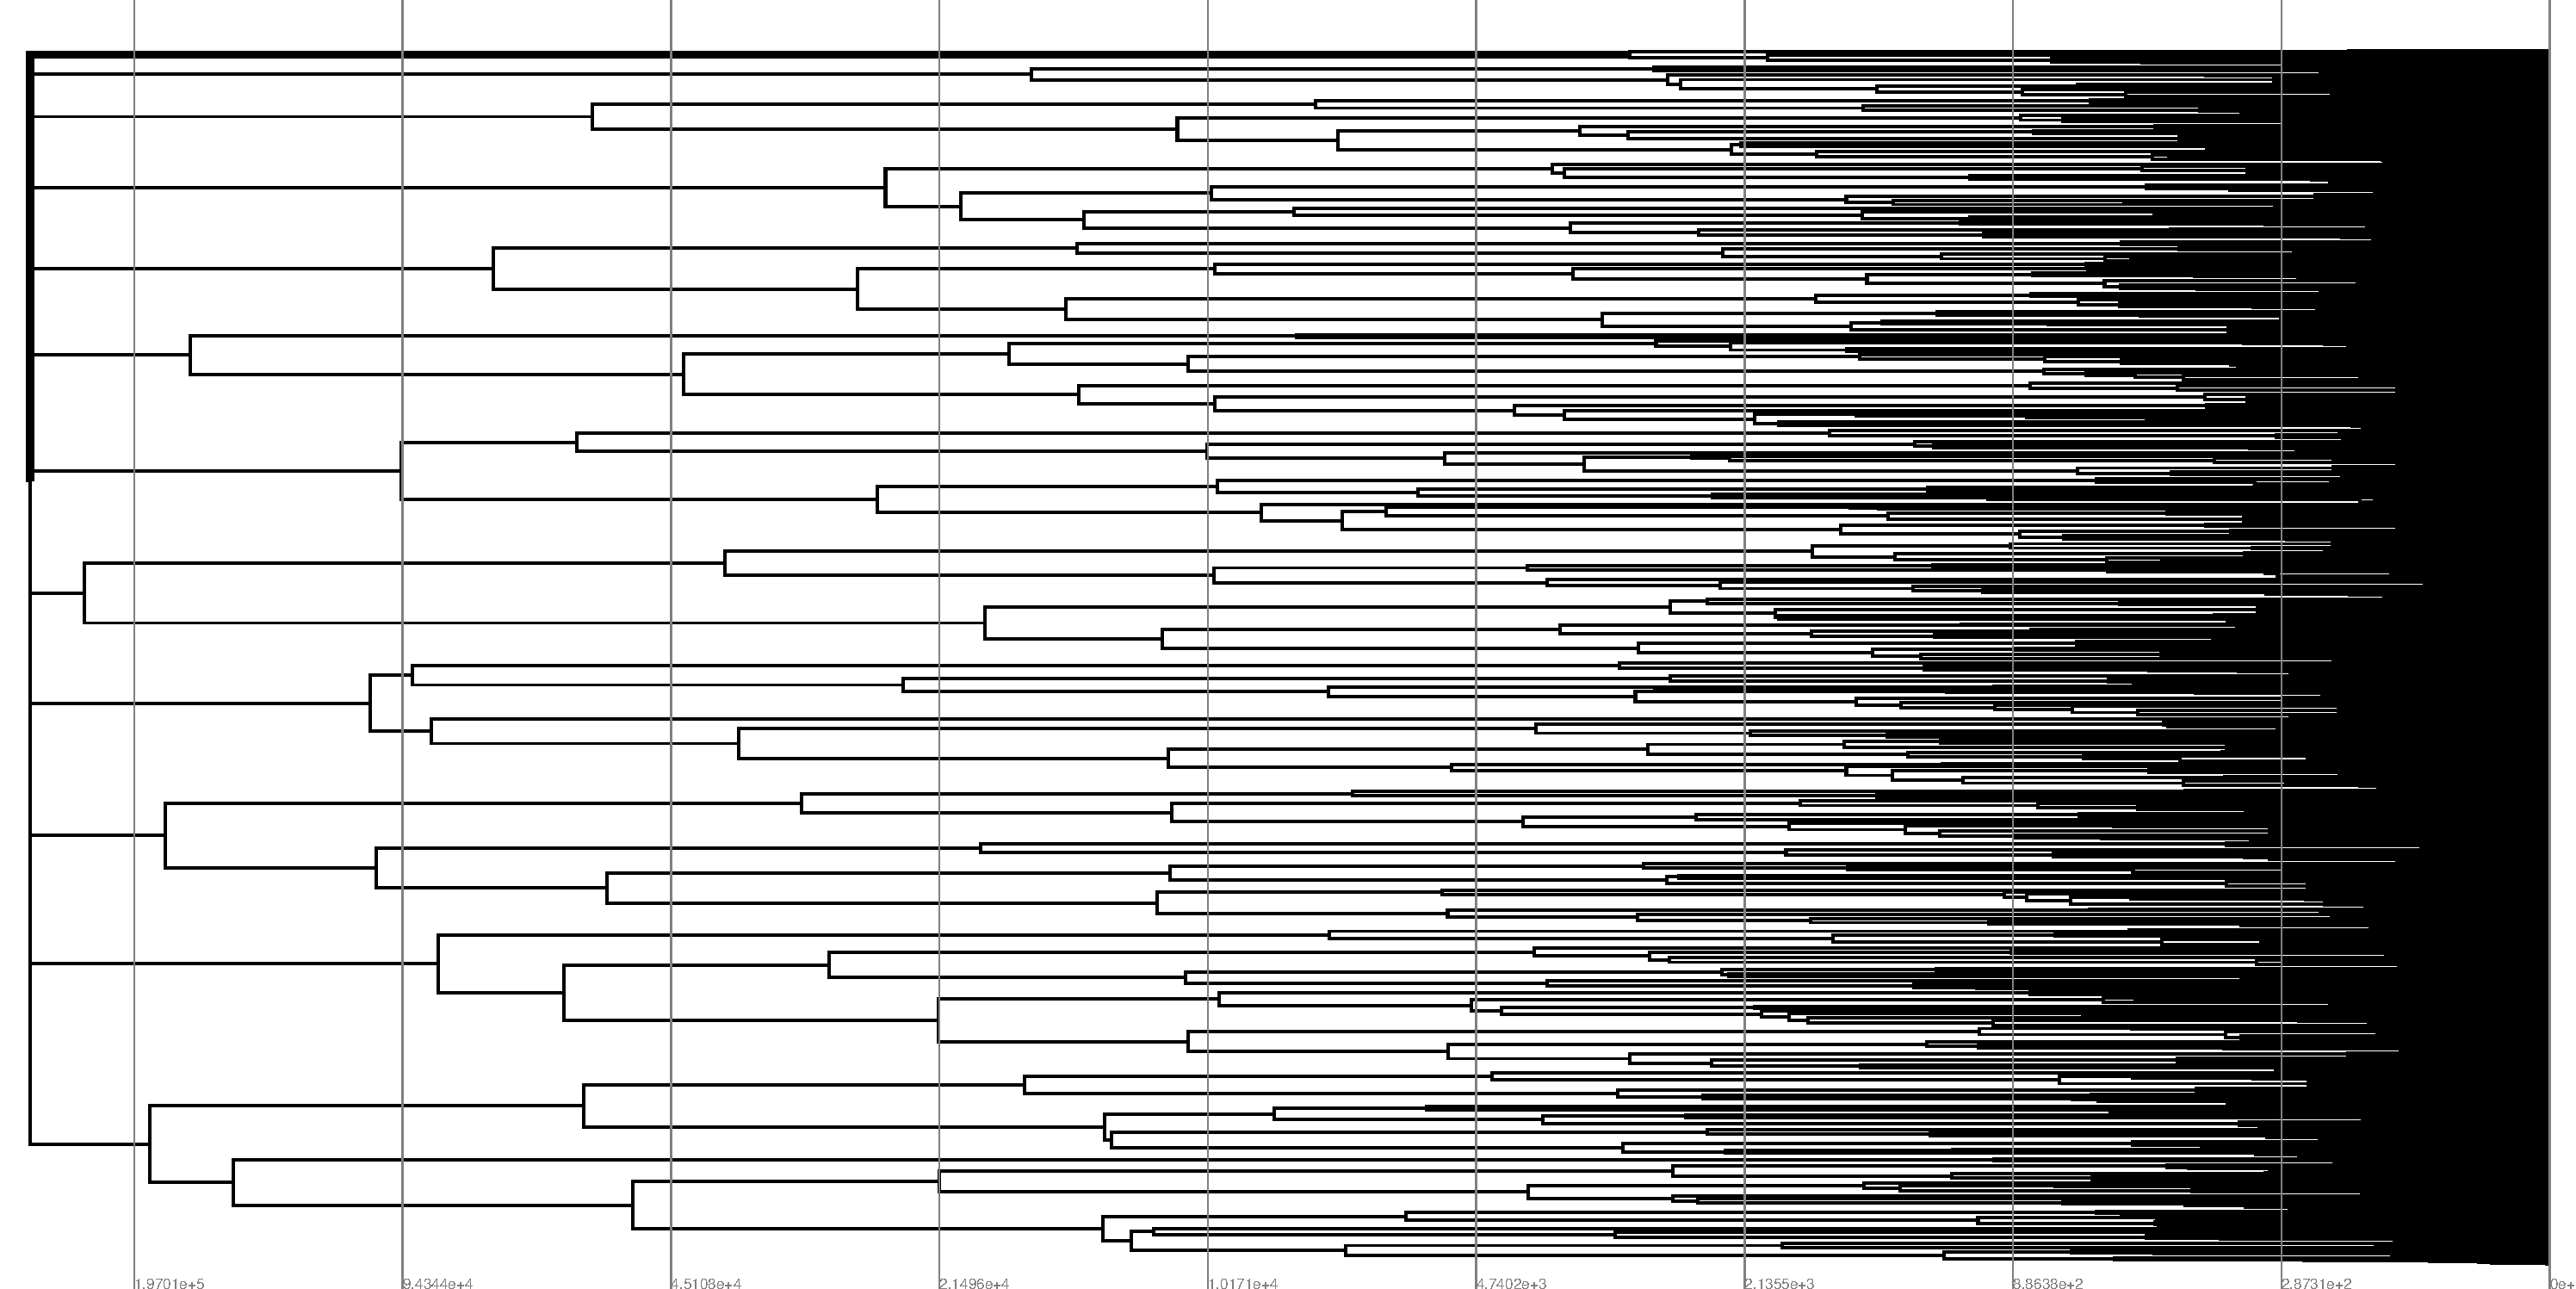
\includegraphics[height=0.12\textheight,width=\textwidth]{img/perfect-tree-phylogenies-log/epoch=7+resolution=3+treatment=12/a=collapsed-phylogeny+epoch=00007+mut_distn=np.random.standard_normal+num_generations=32768+num_islands=1024+num_niches=1+p_island_migration=0.01+p_niche_invasion=3.0517578125e-08+population_size=3276.../8+replicate=0+tournament_size=1+treatment=12+_generation=262144+_index=12+ext=.pdf}
    % \end{noindent}
    \caption{%
      spatial structure weak selection}
    % \label{fig:perfect-tree-phylogenies-log:TODO}
  \end{subfigure}
  \hfill
  \begin{subfigure}[b]{1\columnwidth}
    % \begin{noindent}
    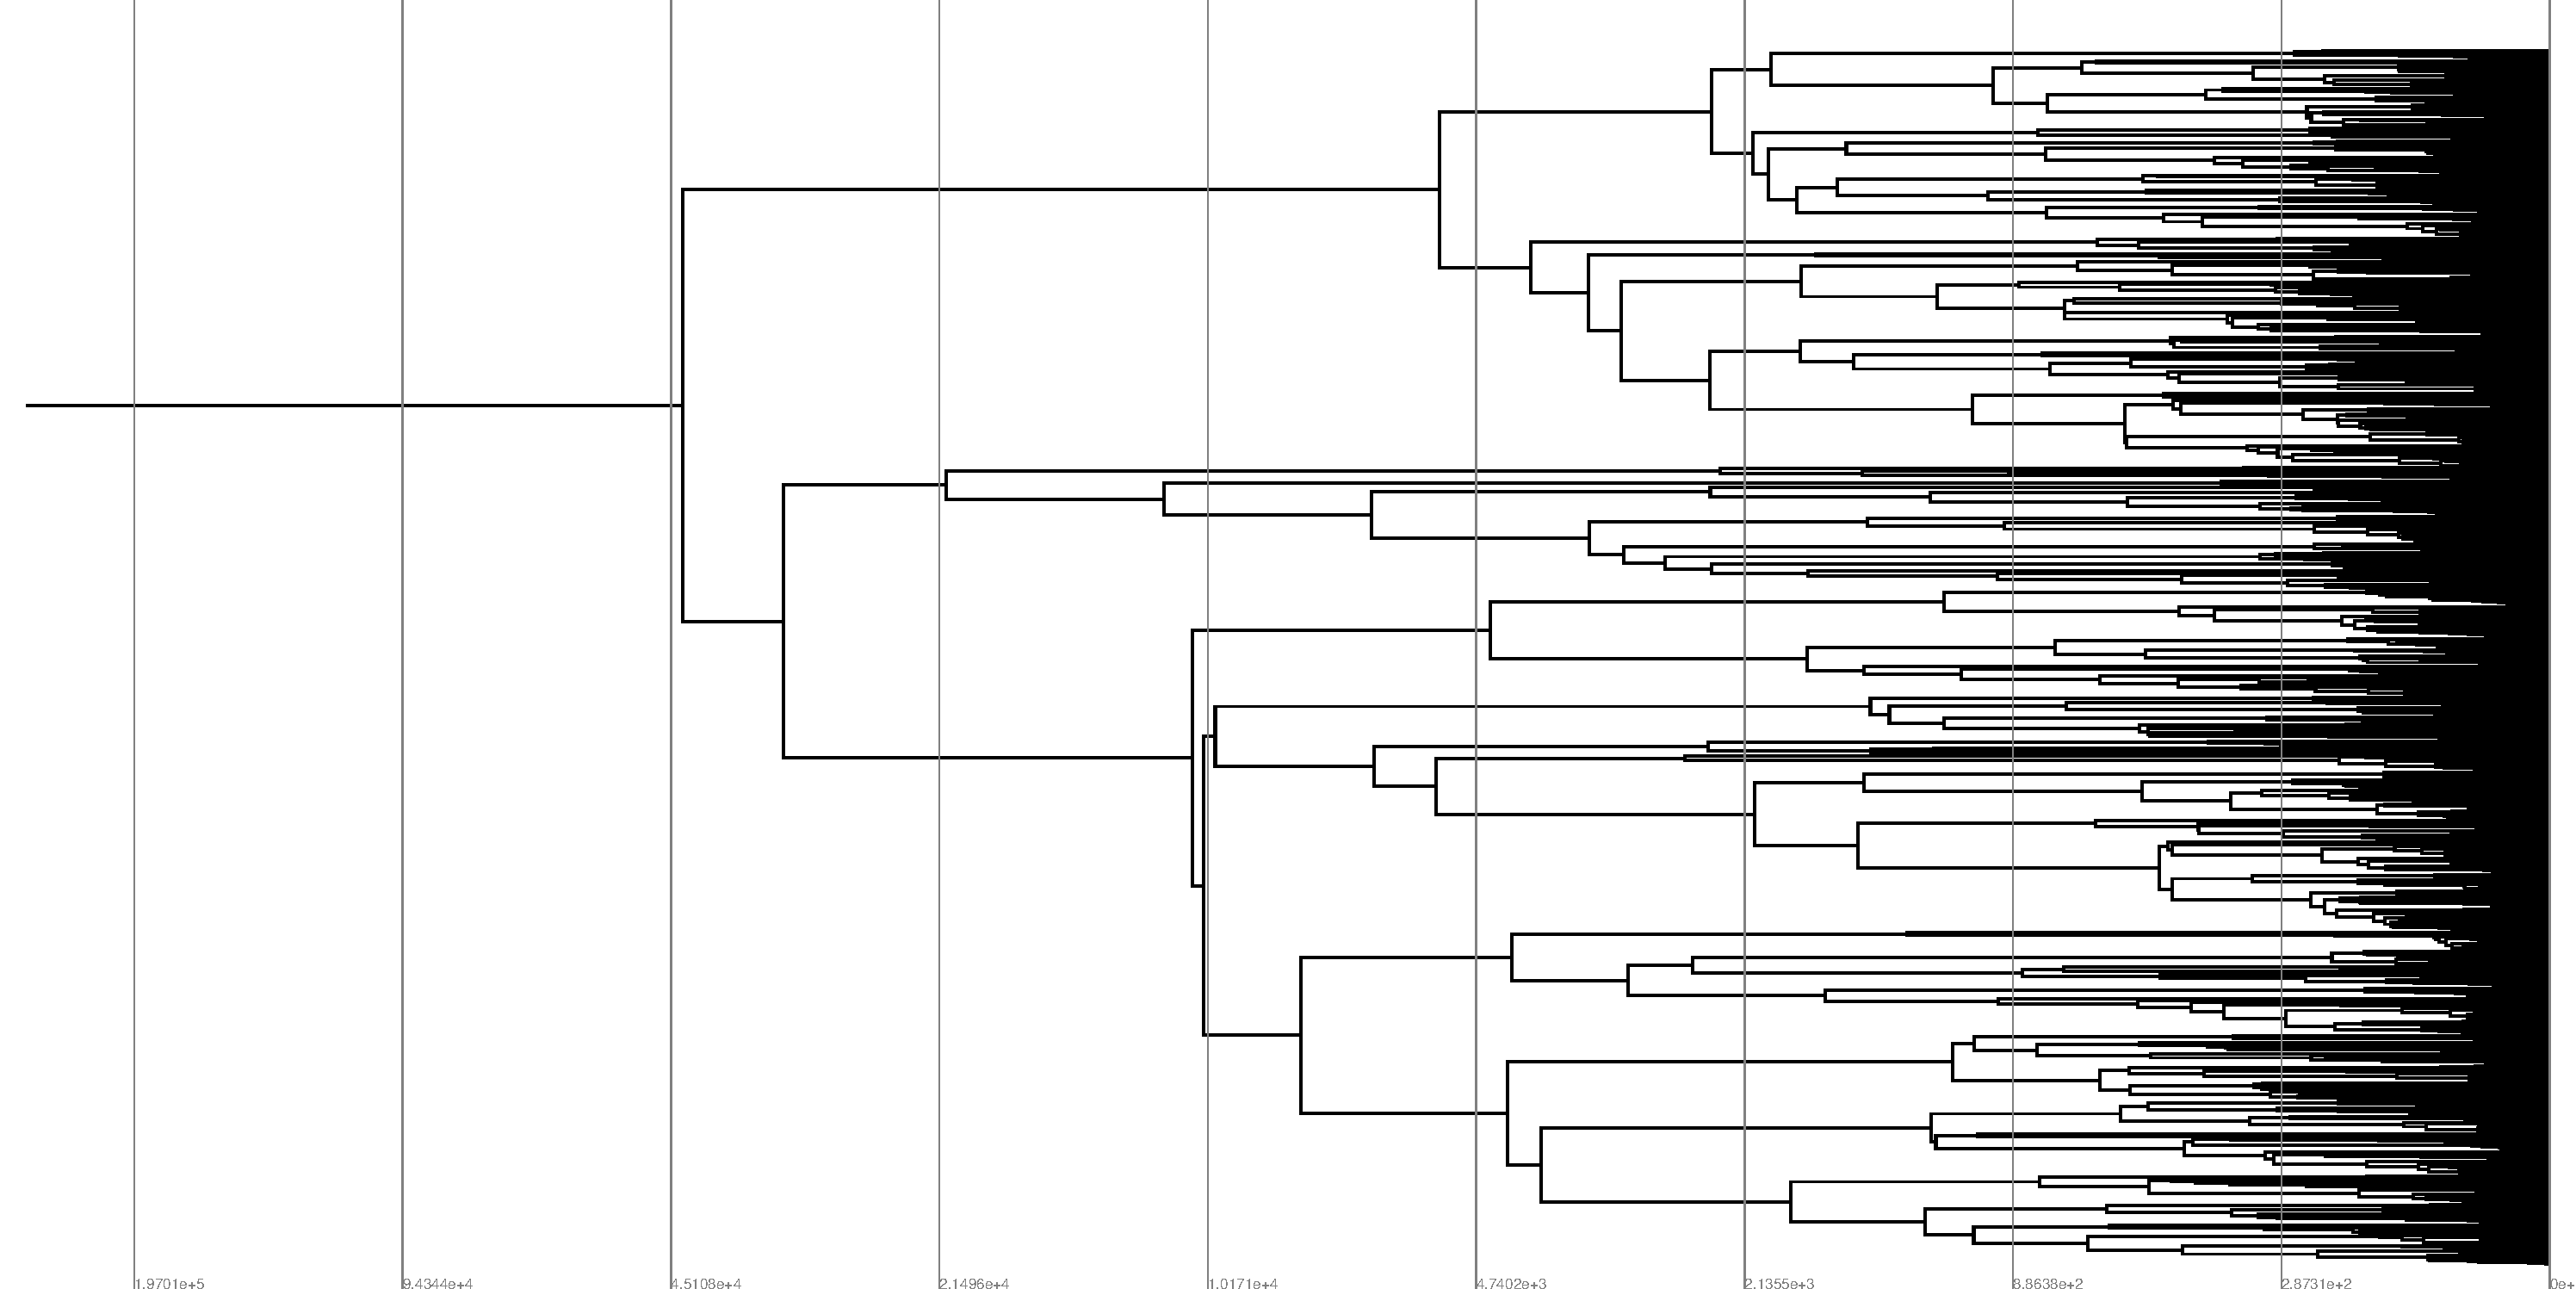
\includegraphics[height=0.12\textheight,width=\textwidth]{img/perfect-tree-phylogenies-log/epoch=7+resolution=3+treatment=14/a=collapsed-phylogeny+epoch=00007+mut_distn=np.random.standard_normal+num_generations=32768+num_islands=1+num_niches=1+p_island_migration=0.01+p_niche_invasion=3.0517578125e-08+population_size=32768+r.../eplicate=0+tournament_size=1+treatment=14+_generation=262144+_index=14+ext=.pdf}
    % \end{noindent}
    \caption{%
      weak selection}
    % \label{fig:perfect-tree-phylogenies-log:TODO}
  \end{subfigure}
  \hfill
  \begin{subfigure}[b]{1\columnwidth}
    % \begin{noindent}
    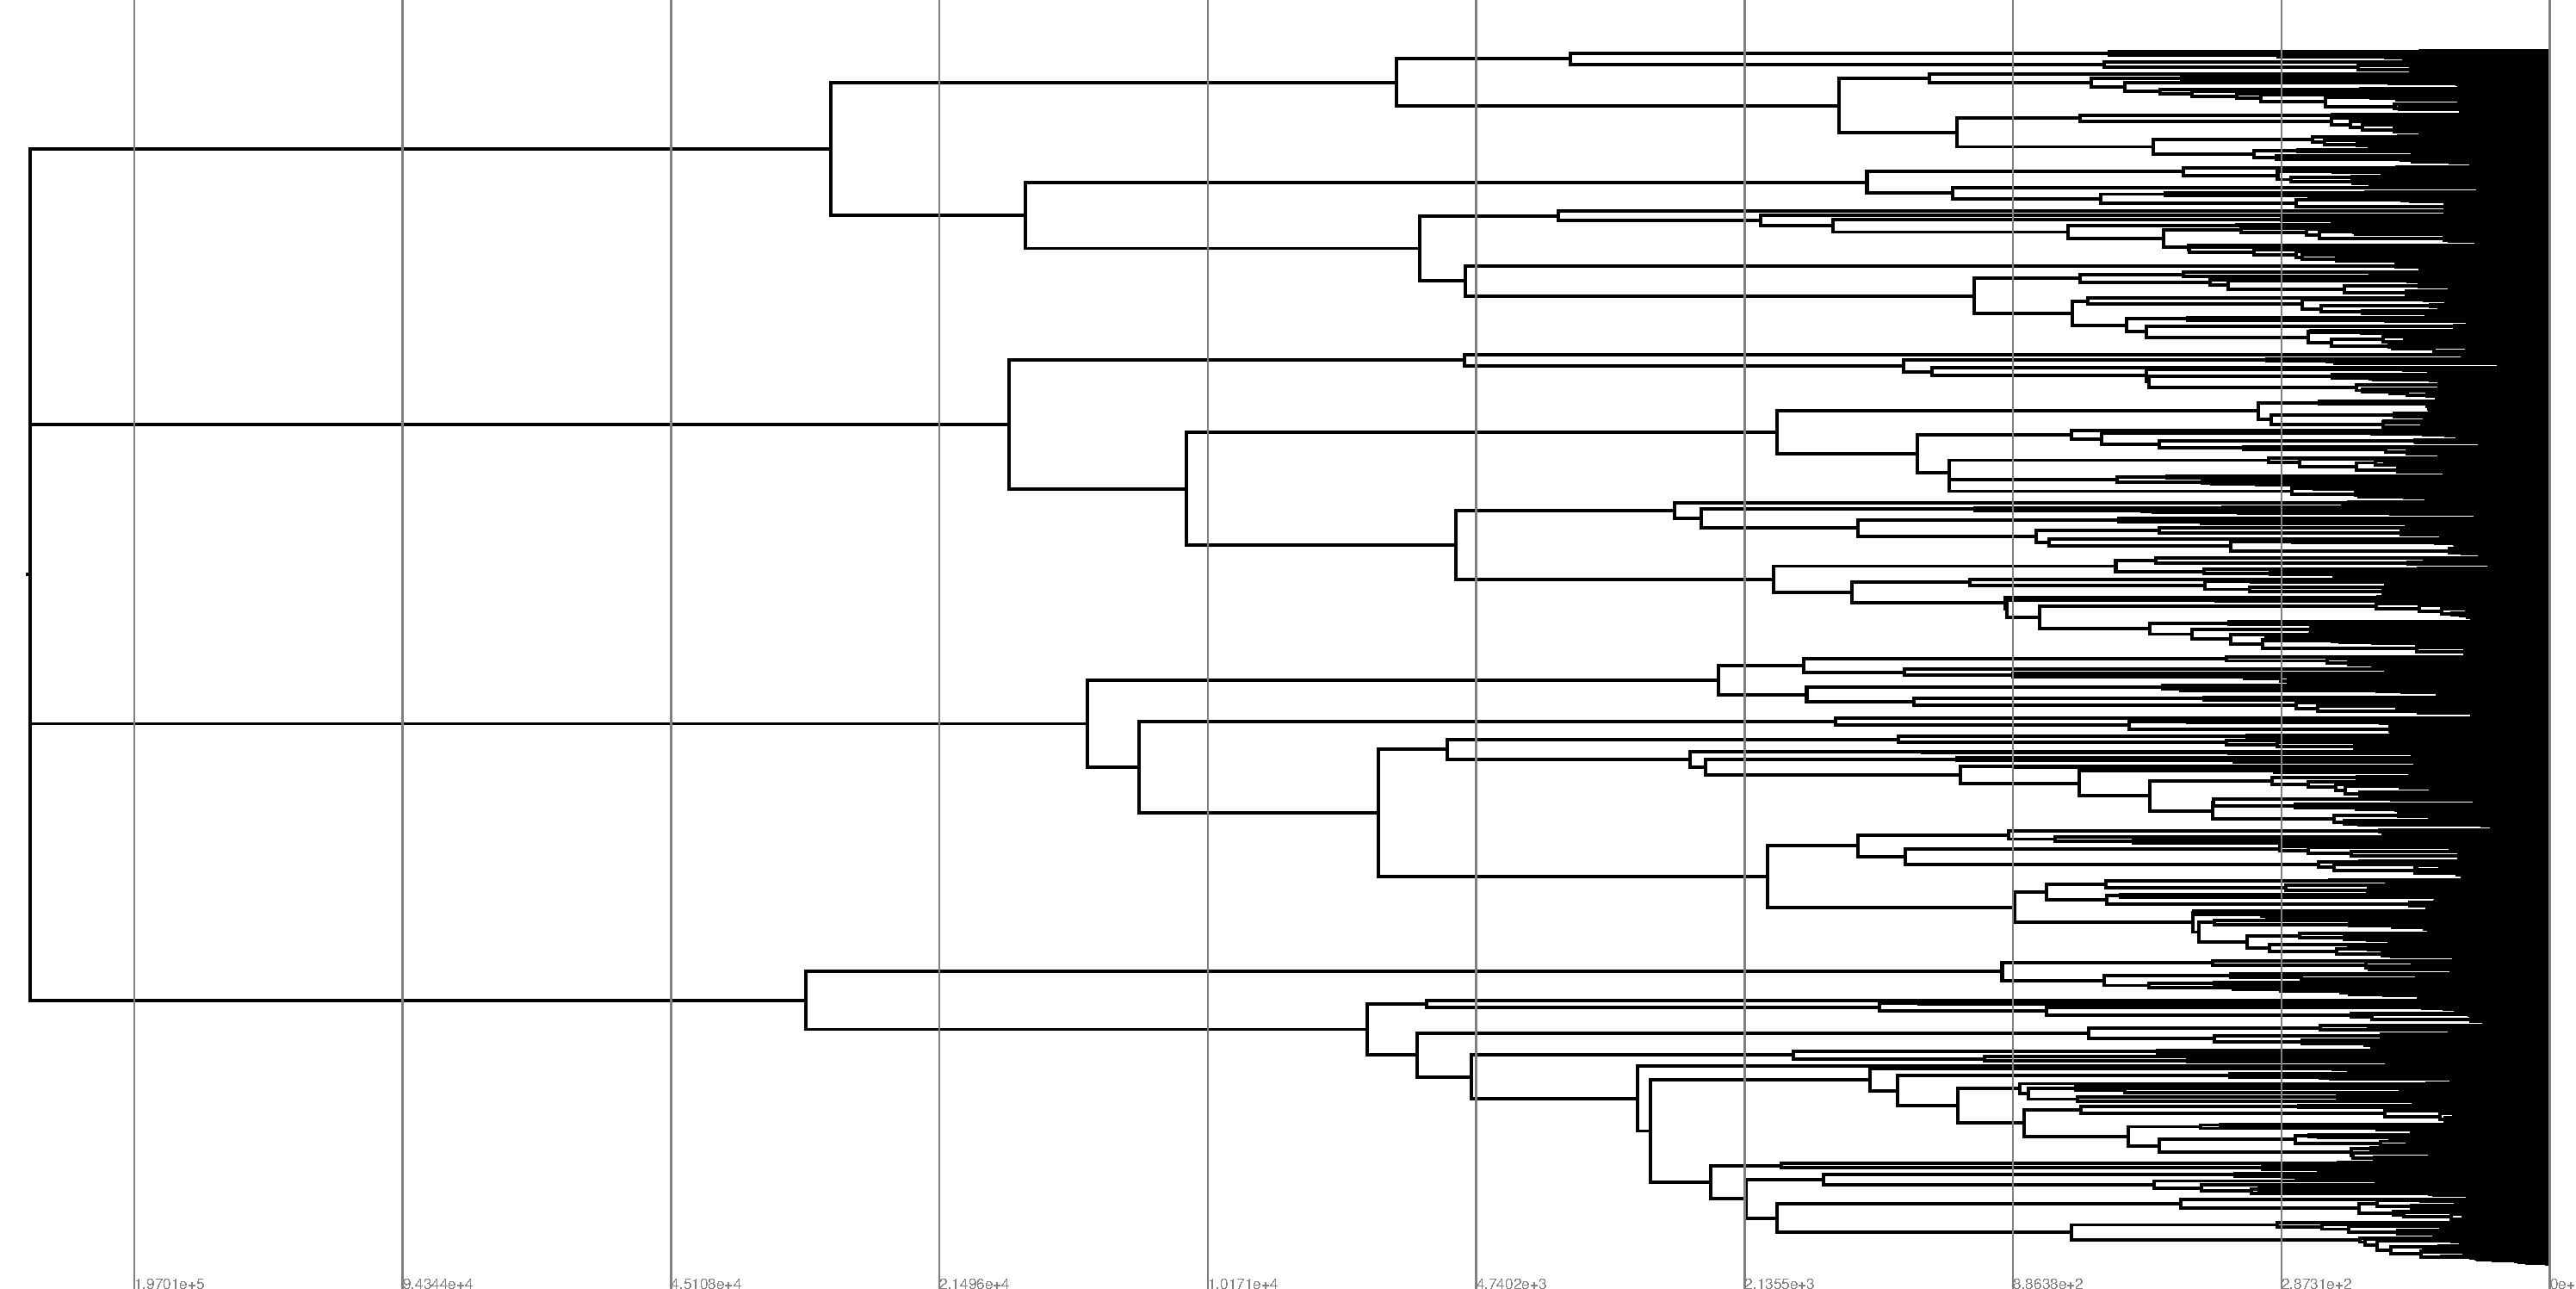
\includegraphics[height=0.12\textheight,width=\textwidth]{img/perfect-tree-phylogenies-log/epoch=7+resolution=3+treatment=16/a=collapsed-phylogeny+epoch=00007+mut_distn=np.random.standard_normal+num_generations=32768+num_islands=1+num_niches=4+p_island_migration=0.01+p_niche_invasion=3.0517578125e-08+population_size=32768+r.../eplicate=0+tournament_size=1+treatment=16+_generation=262144+_index=16+ext=.pdf}
    % \end{noindent}
    \caption{%
      weak selection 4 niche ecology}
    % \label{fig:perfect-tree-phylogenies-log:TODO}
  \end{subfigure}
  \hfill
  \begin{subfigure}[b]{1\columnwidth}
    % \begin{noindent}
    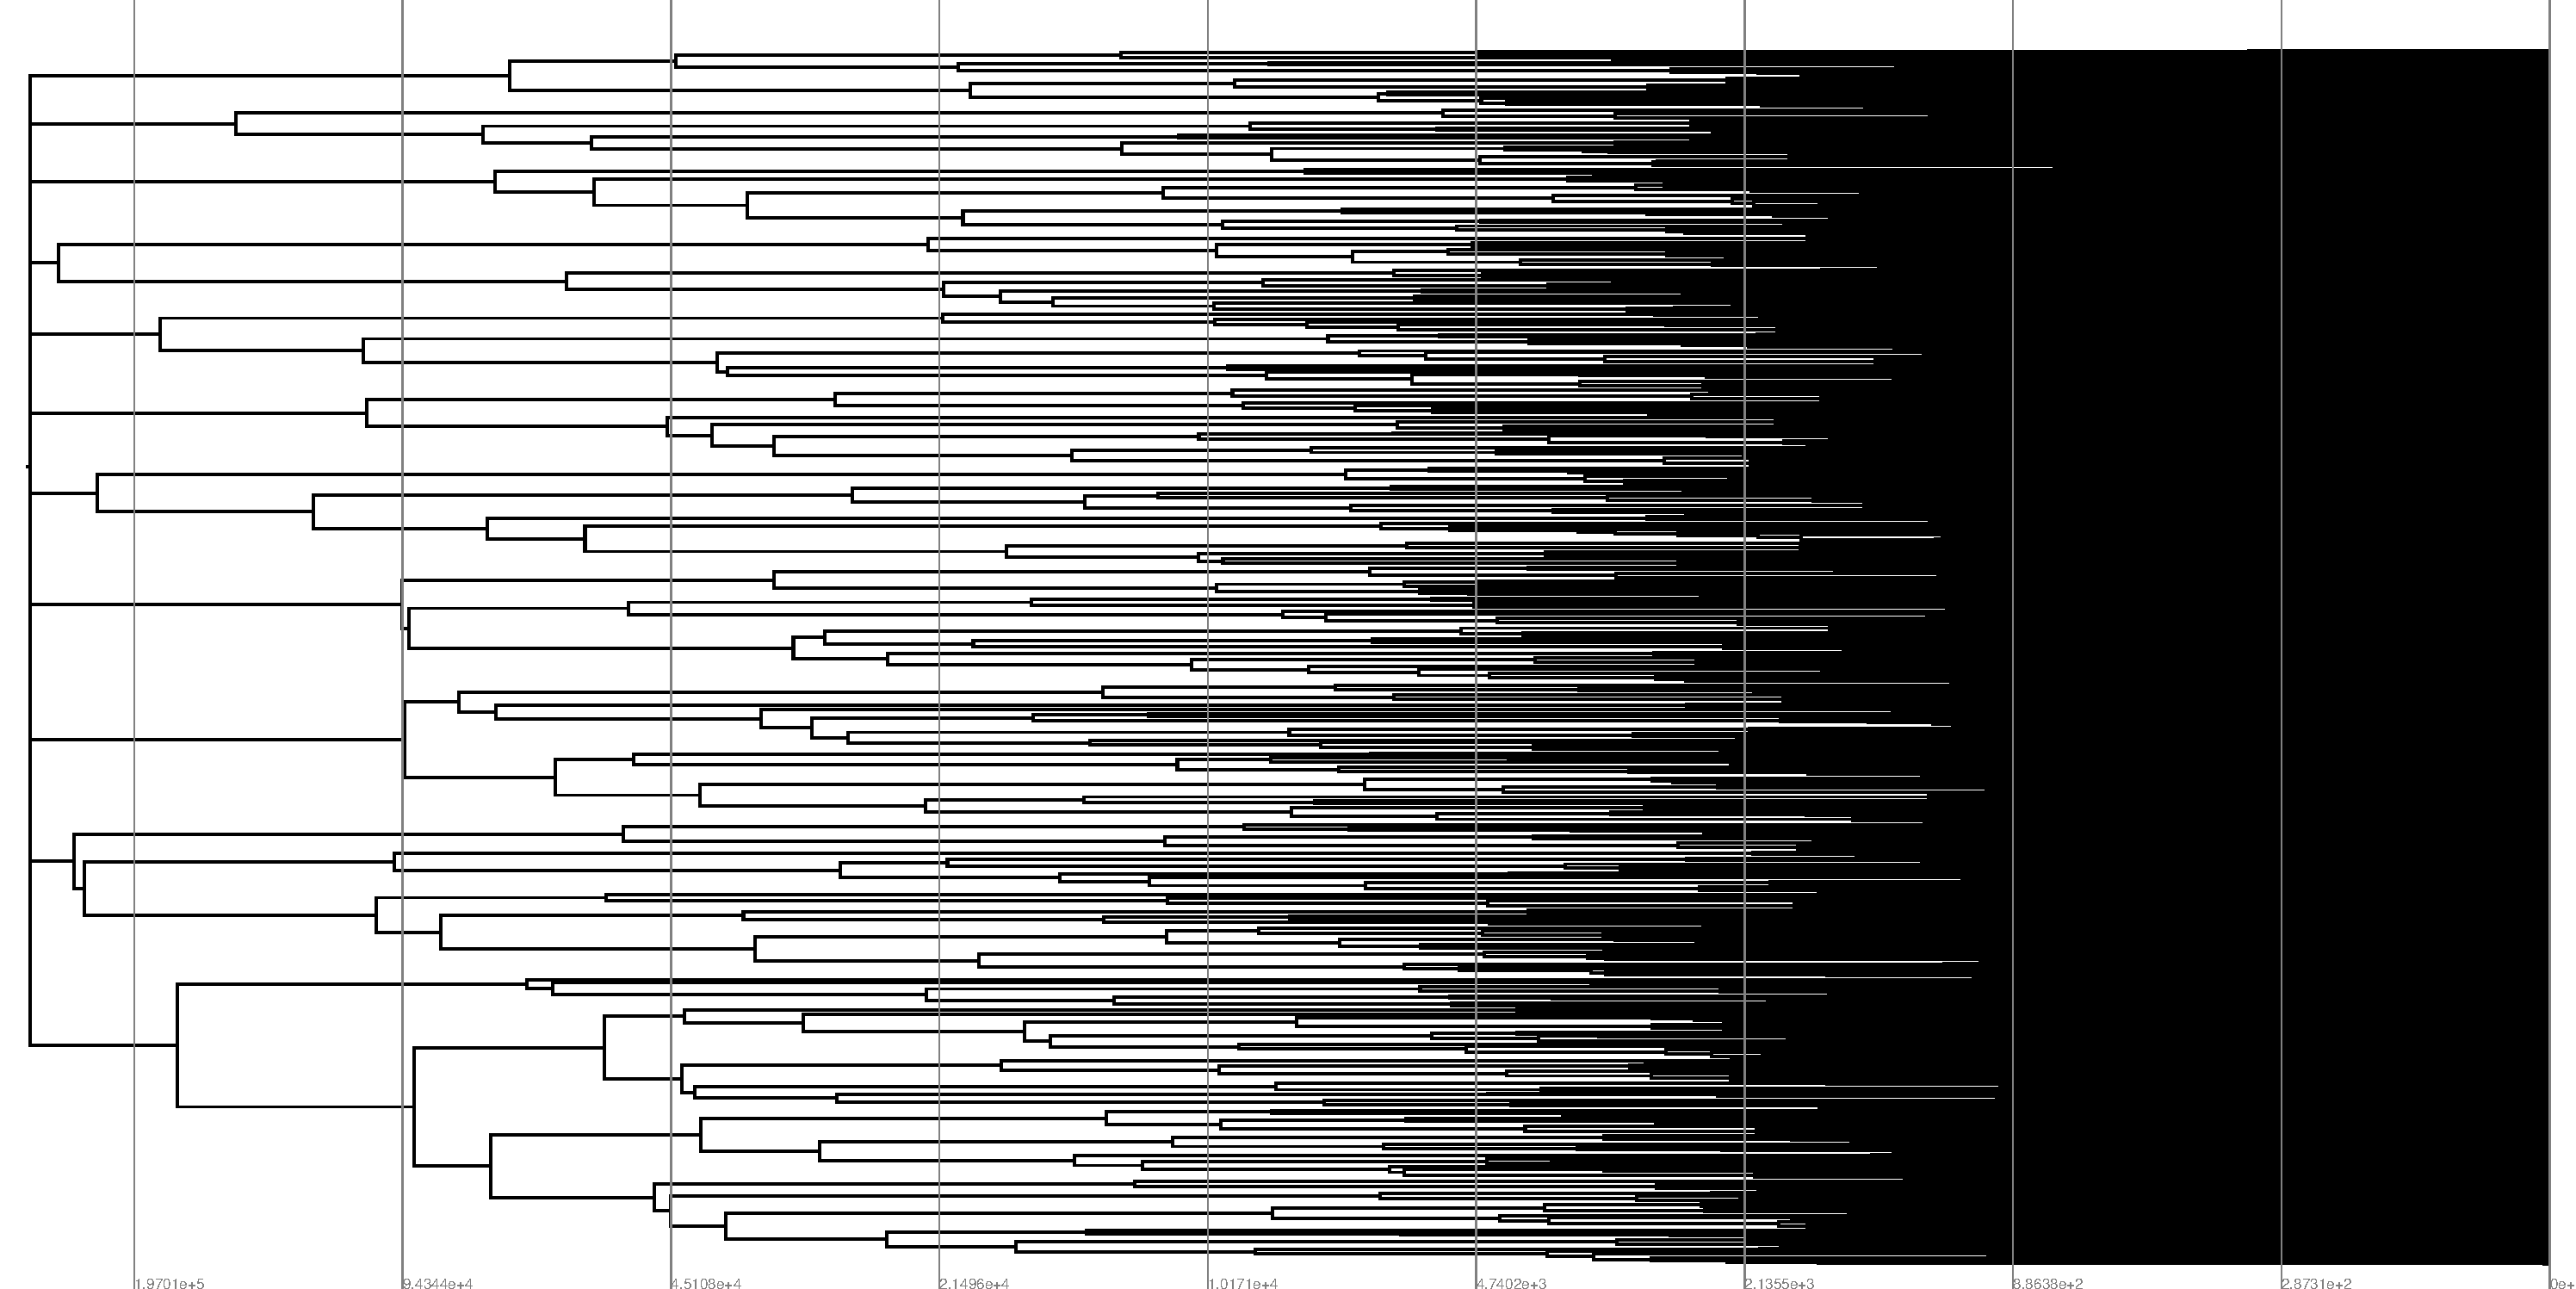
\includegraphics[height=0.12\textheight,width=\textwidth]{img/perfect-tree-phylogenies-log/epoch=7+resolution=3+treatment=18/a=collapsed-phylogeny+epoch=00007+mut_distn=np.random.standard_normal+num_generations=32768+num_islands=1024+num_niches=8+p_island_migration=0.01+p_niche_invasion=3.0517578125e-08+population_size=3276.../8+replicate=0+tournament_size=2+treatment=18+_generation=262144+_index=18+ext=.pdf}
    % \end{noindent}
    \caption{%
      spatial structure 8 niche ecology}
    % \label{fig:perfect-tree-phylogenies-log:TODO}
  \end{subfigure}

  \begin{subfigure}[b]{1\columnwidth}
    % \begin{noindent}
    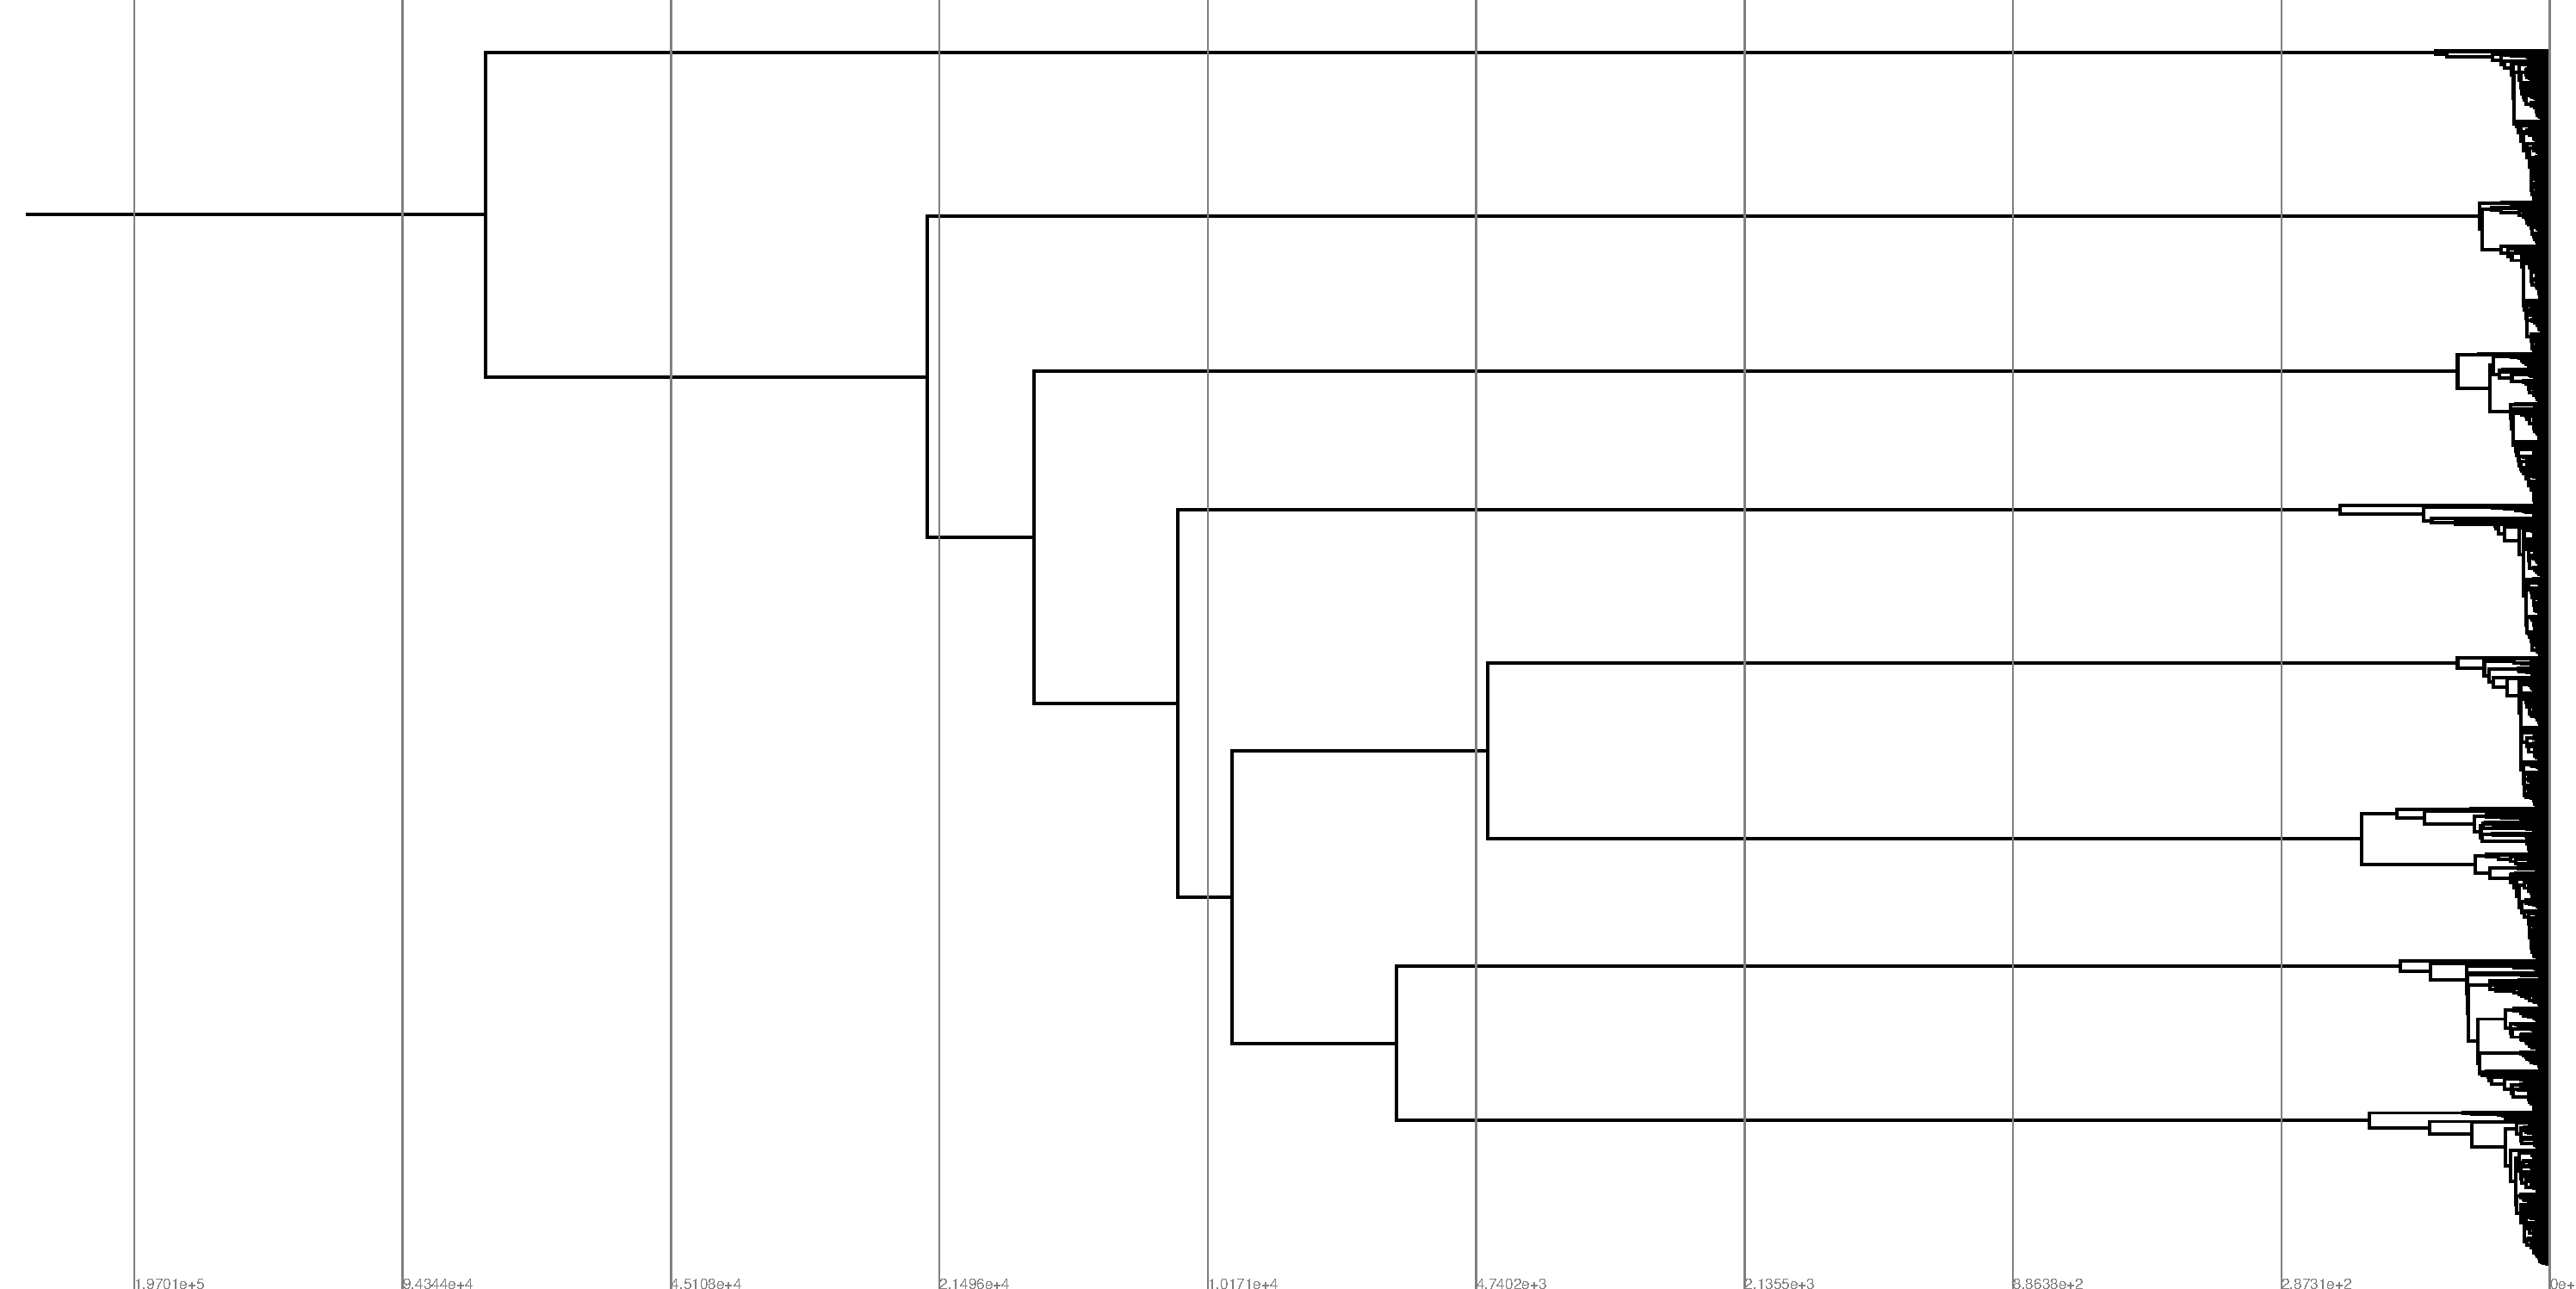
\includegraphics[height=0.12\textheight,width=\textwidth]{img/perfect-tree-phylogenies-log/epoch=7+resolution=3+treatment=20/a=collapsed-phylogeny+epoch=00007+mut_distn=np.random.standard_normal+num_generations=32768+num_islands=1+num_niches=8+p_island_migration=0.01+p_niche_invasion=3.0517578125e-08+population_size=32768+r.../eplicate=0+tournament_size=2+treatment=20+_generation=262144+_index=20+ext=.pdf}
    % \end{noindent}
    \caption{%
      8 niche ecology}
    % \label{fig:perfect-tree-phylogenies-log:TODO}
  \end{subfigure}
  \hfill
  \begin{subfigure}[b]{1\columnwidth}
    % \begin{noindent}
    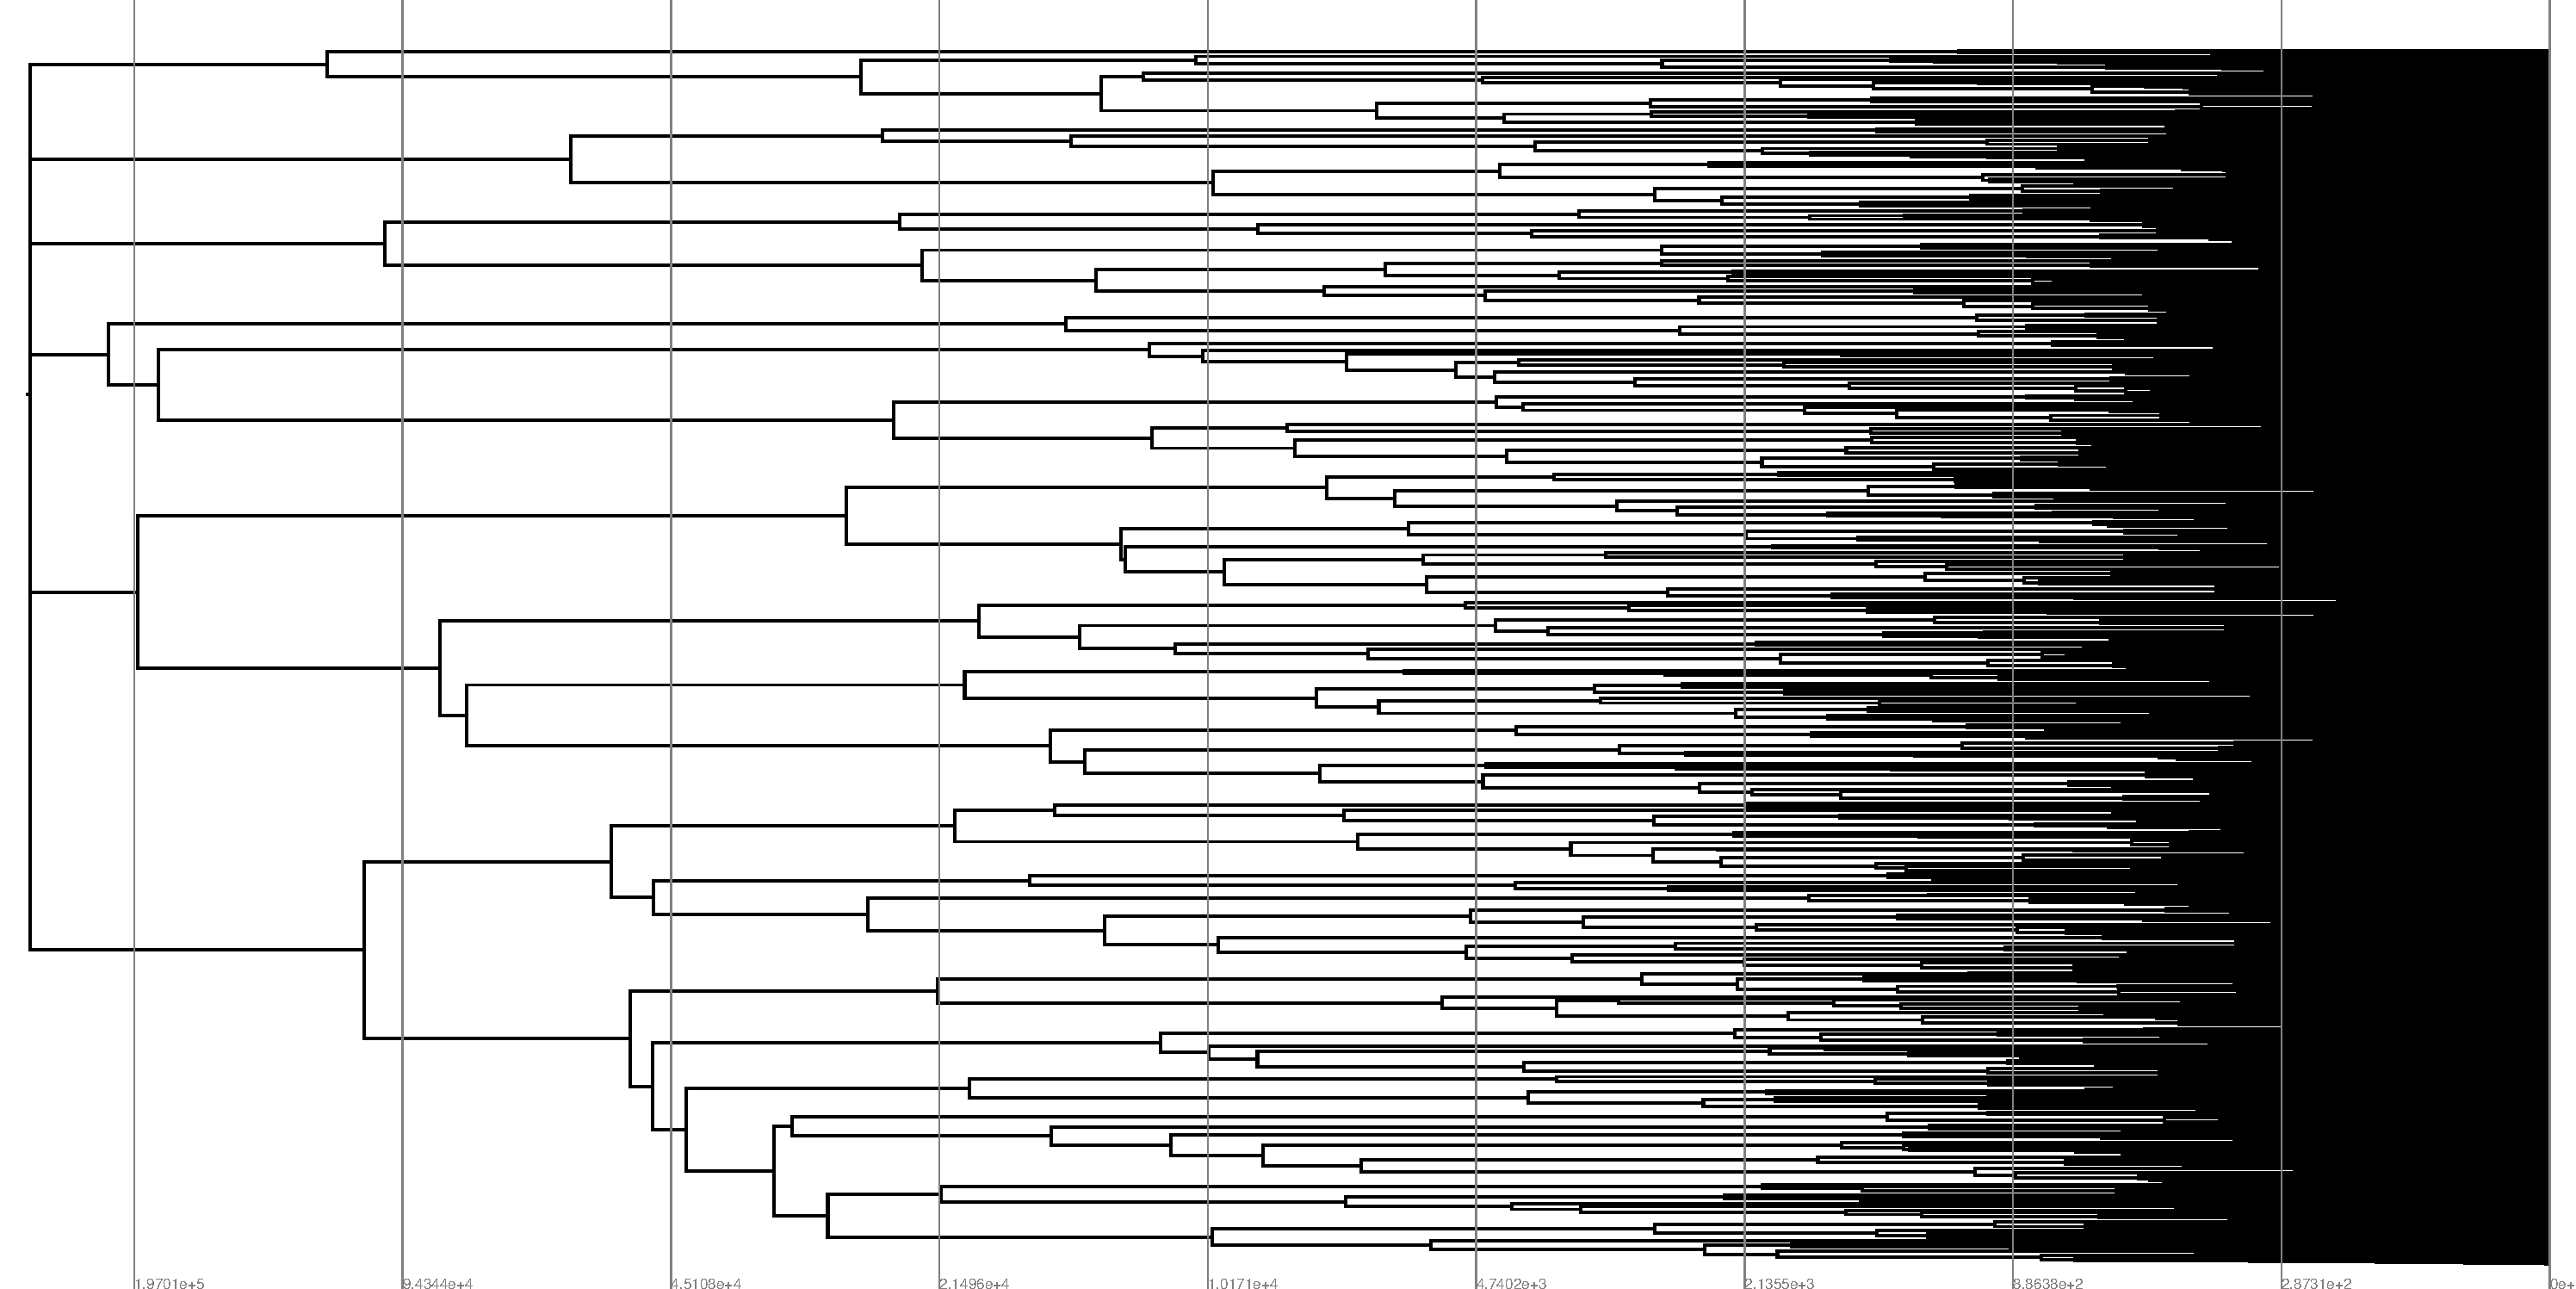
\includegraphics[height=0.12\textheight,width=\textwidth]{img/perfect-tree-phylogenies-log/epoch=7+resolution=3+treatment=22/a=collapsed-phylogeny+epoch=00007+mut_distn=np.random.standard_normal+num_generations=32768+num_islands=1024+num_niches=4+p_island_migration=0.01+p_niche_invasion=3.0517578125e-08+population_size=3276.../8+replicate=0+tournament_size=2+treatment=22+_generation=262144+_index=22+ext=.pdf}
    % \end{noindent}
    \caption{%
      spatial structure 4 niche ecology}
    % \label{fig:perfect-tree-phylogenies-log:TODO}
  \end{subfigure}
  \hfill
  \begin{subfigure}[b]{1\columnwidth}
    % \begin{noindent}
    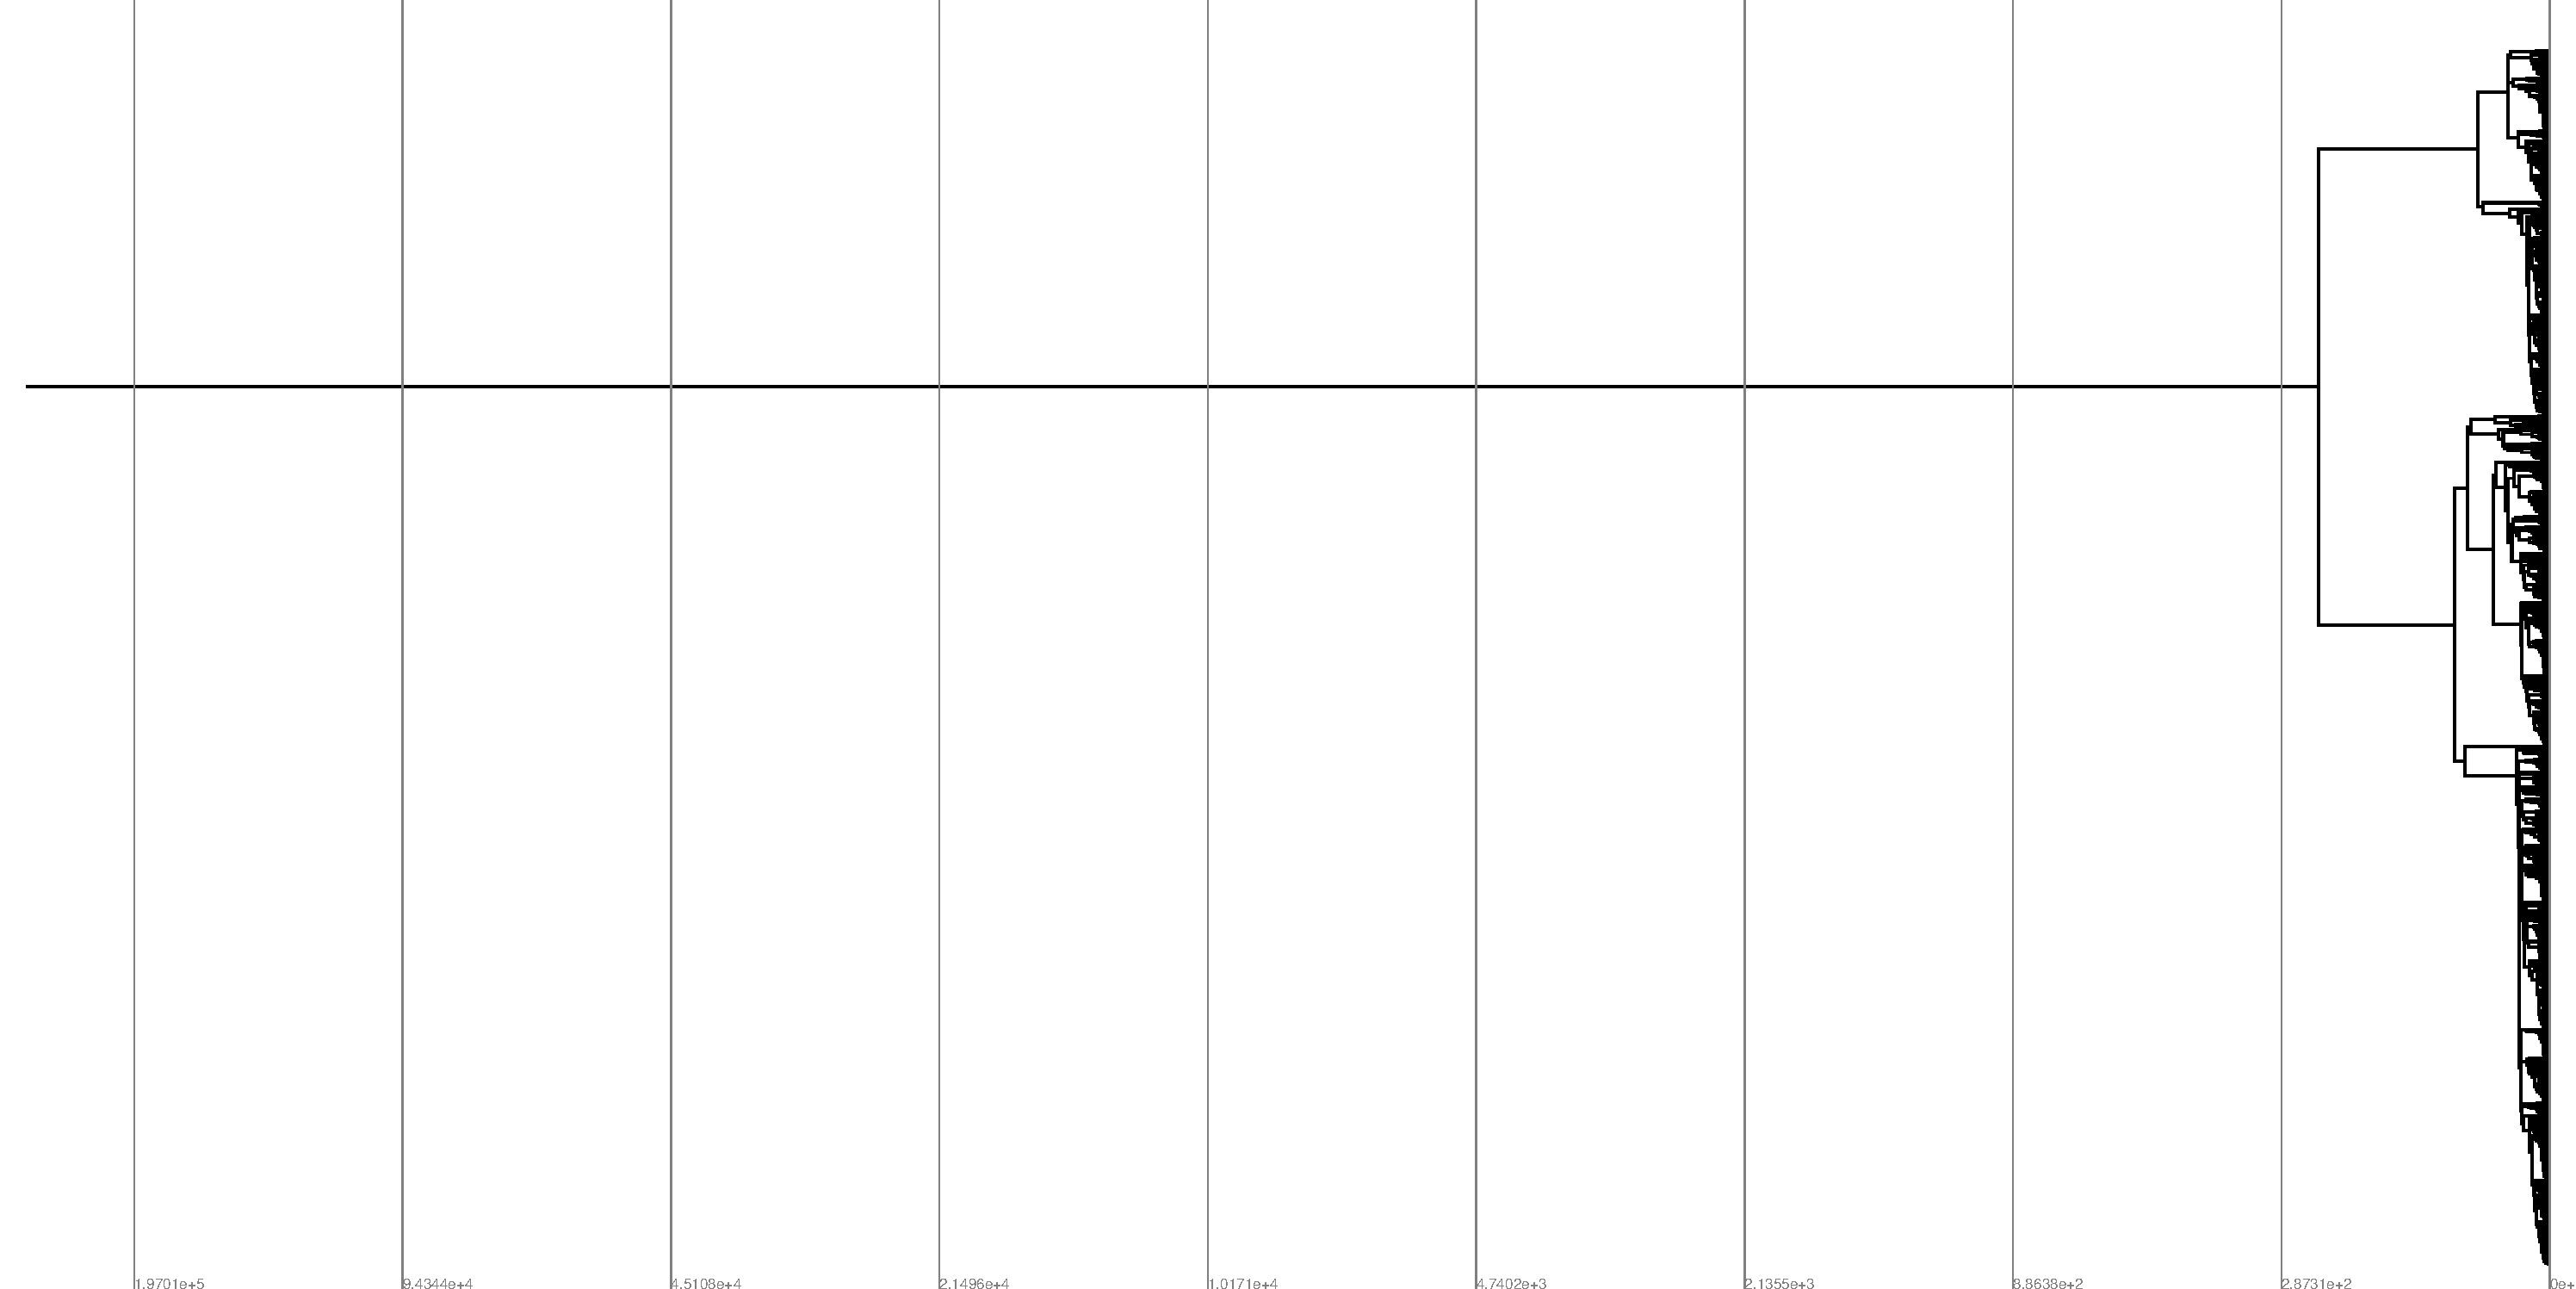
\includegraphics[height=0.12\textheight,width=\textwidth]{img/perfect-tree-phylogenies-log/epoch=7+resolution=3+treatment=2/a=collapsed-phylogeny+epoch=00007+mut_distn=np.random.standard_normal+num_generations=32768+num_islands=1+num_niches=1+p_island_migration=0.01+p_niche_invasion=3.0517578125e-08+population_size=32768+r.../eplicate=0+tournament_size=4+treatment=2+_generation=262144+_index=2+ext=.pdf}
    % \end{noindent}
    \caption{%
      strong selection}
    % \label{fig:perfect-tree-phylogenies-log:TODO}
  \end{subfigure}
  \hfill
  \begin{subfigure}[b]{1\columnwidth}
    % \begin{noindent}
    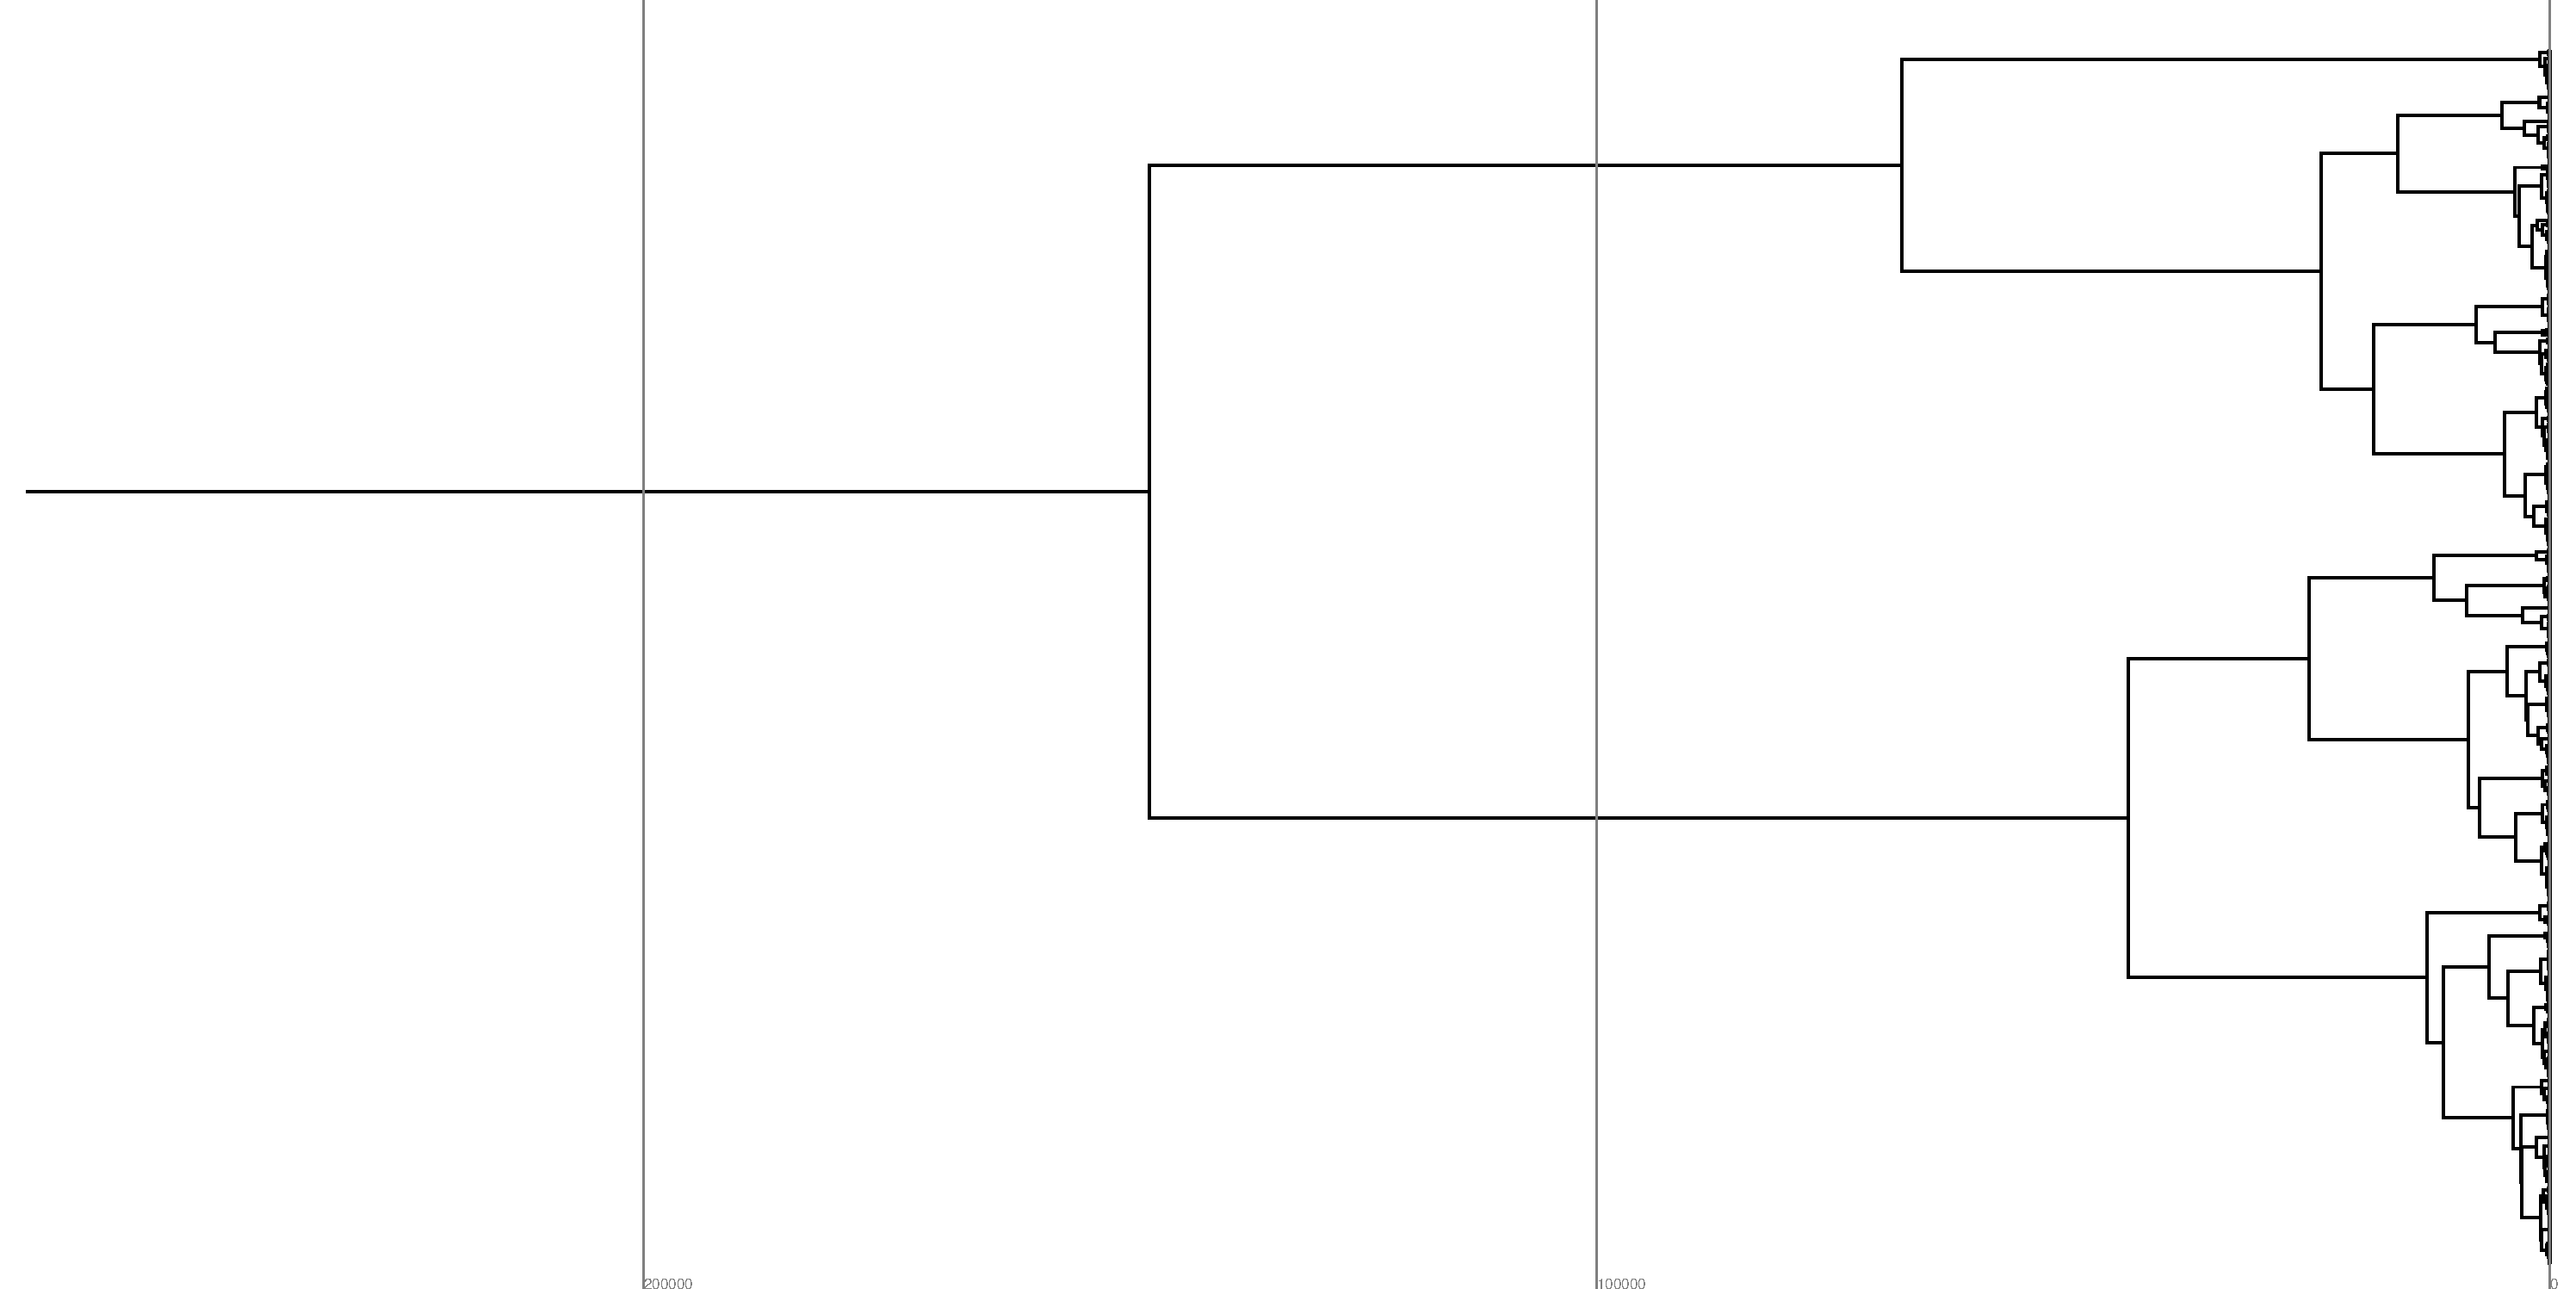
\includegraphics[height=0.12\textheight,width=\textwidth]{img/perfect-tree-phylogenies-log/epoch=7+resolution=3+treatment=4/a=collapsed-phylogeny+epoch=00007+mut_distn=np.random.standard_normal+num_generations=32768+num_islands=1+num_niches=4+p_island_migration=0.01+p_niche_invasion=3.0517578125e-08+population_size=32768+r.../eplicate=0+tournament_size=4+treatment=4+_generation=262144+_index=4+ext=.pdf}
    % \end{noindent}
    \caption{%
      4 niche ecology strong selection}
    % \label{fig:perfect-tree-phylogenies-log:TODO}
  \end{subfigure}
  \hfill
  \begin{subfigure}[b]{1\columnwidth}
    % \begin{noindent}
    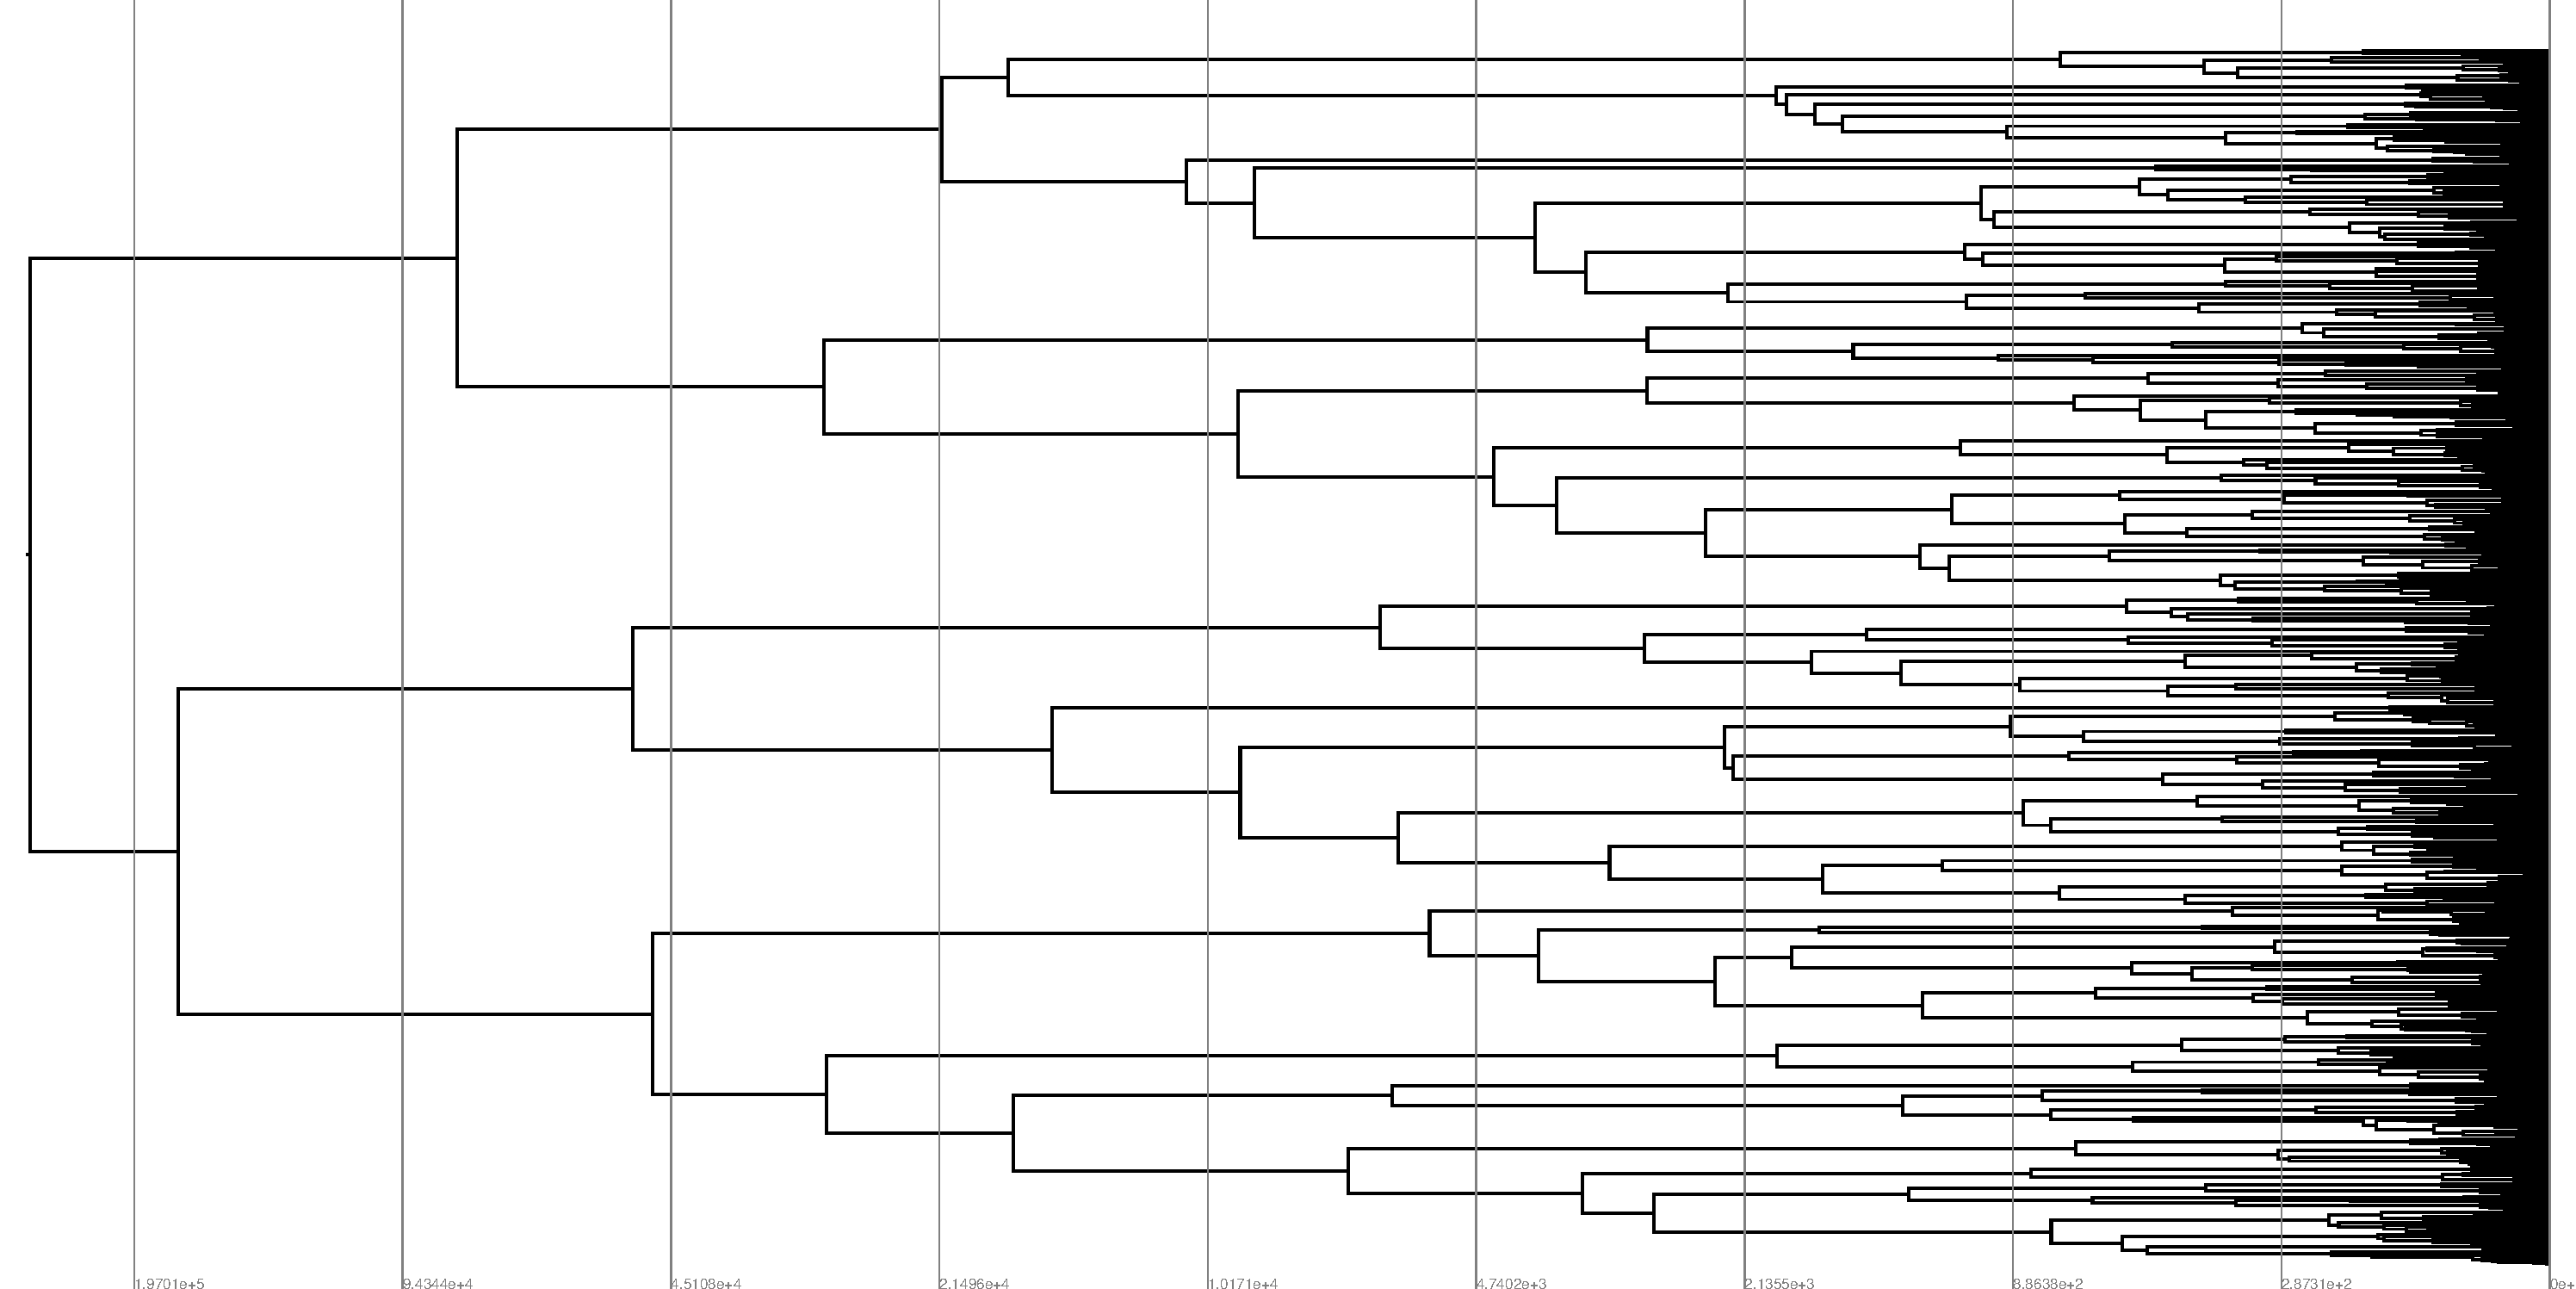
\includegraphics[height=0.12\textheight,width=\textwidth]{img/perfect-tree-phylogenies-log/epoch=7+resolution=3+treatment=6/a=collapsed-phylogeny+epoch=00007+mut_distn=np.random.standard_normal+num_generations=32768+num_islands=1024+num_niches=1+p_island_migration=0.01+p_niche_invasion=3.0517578125e-08+population_size=3276.../8+replicate=0+tournament_size=2+treatment=6+_generation=262144+_index=6+ext=.pdf}
    % \end{noindent}
    \caption{%
      spatial structure}
    % \label{fig:perfect-tree-phylogenies-log:TODO}
  \end{subfigure}
  \hfill
  \begin{subfigure}[b]{1\columnwidth}
    \centering
    % \begin{noindent}
    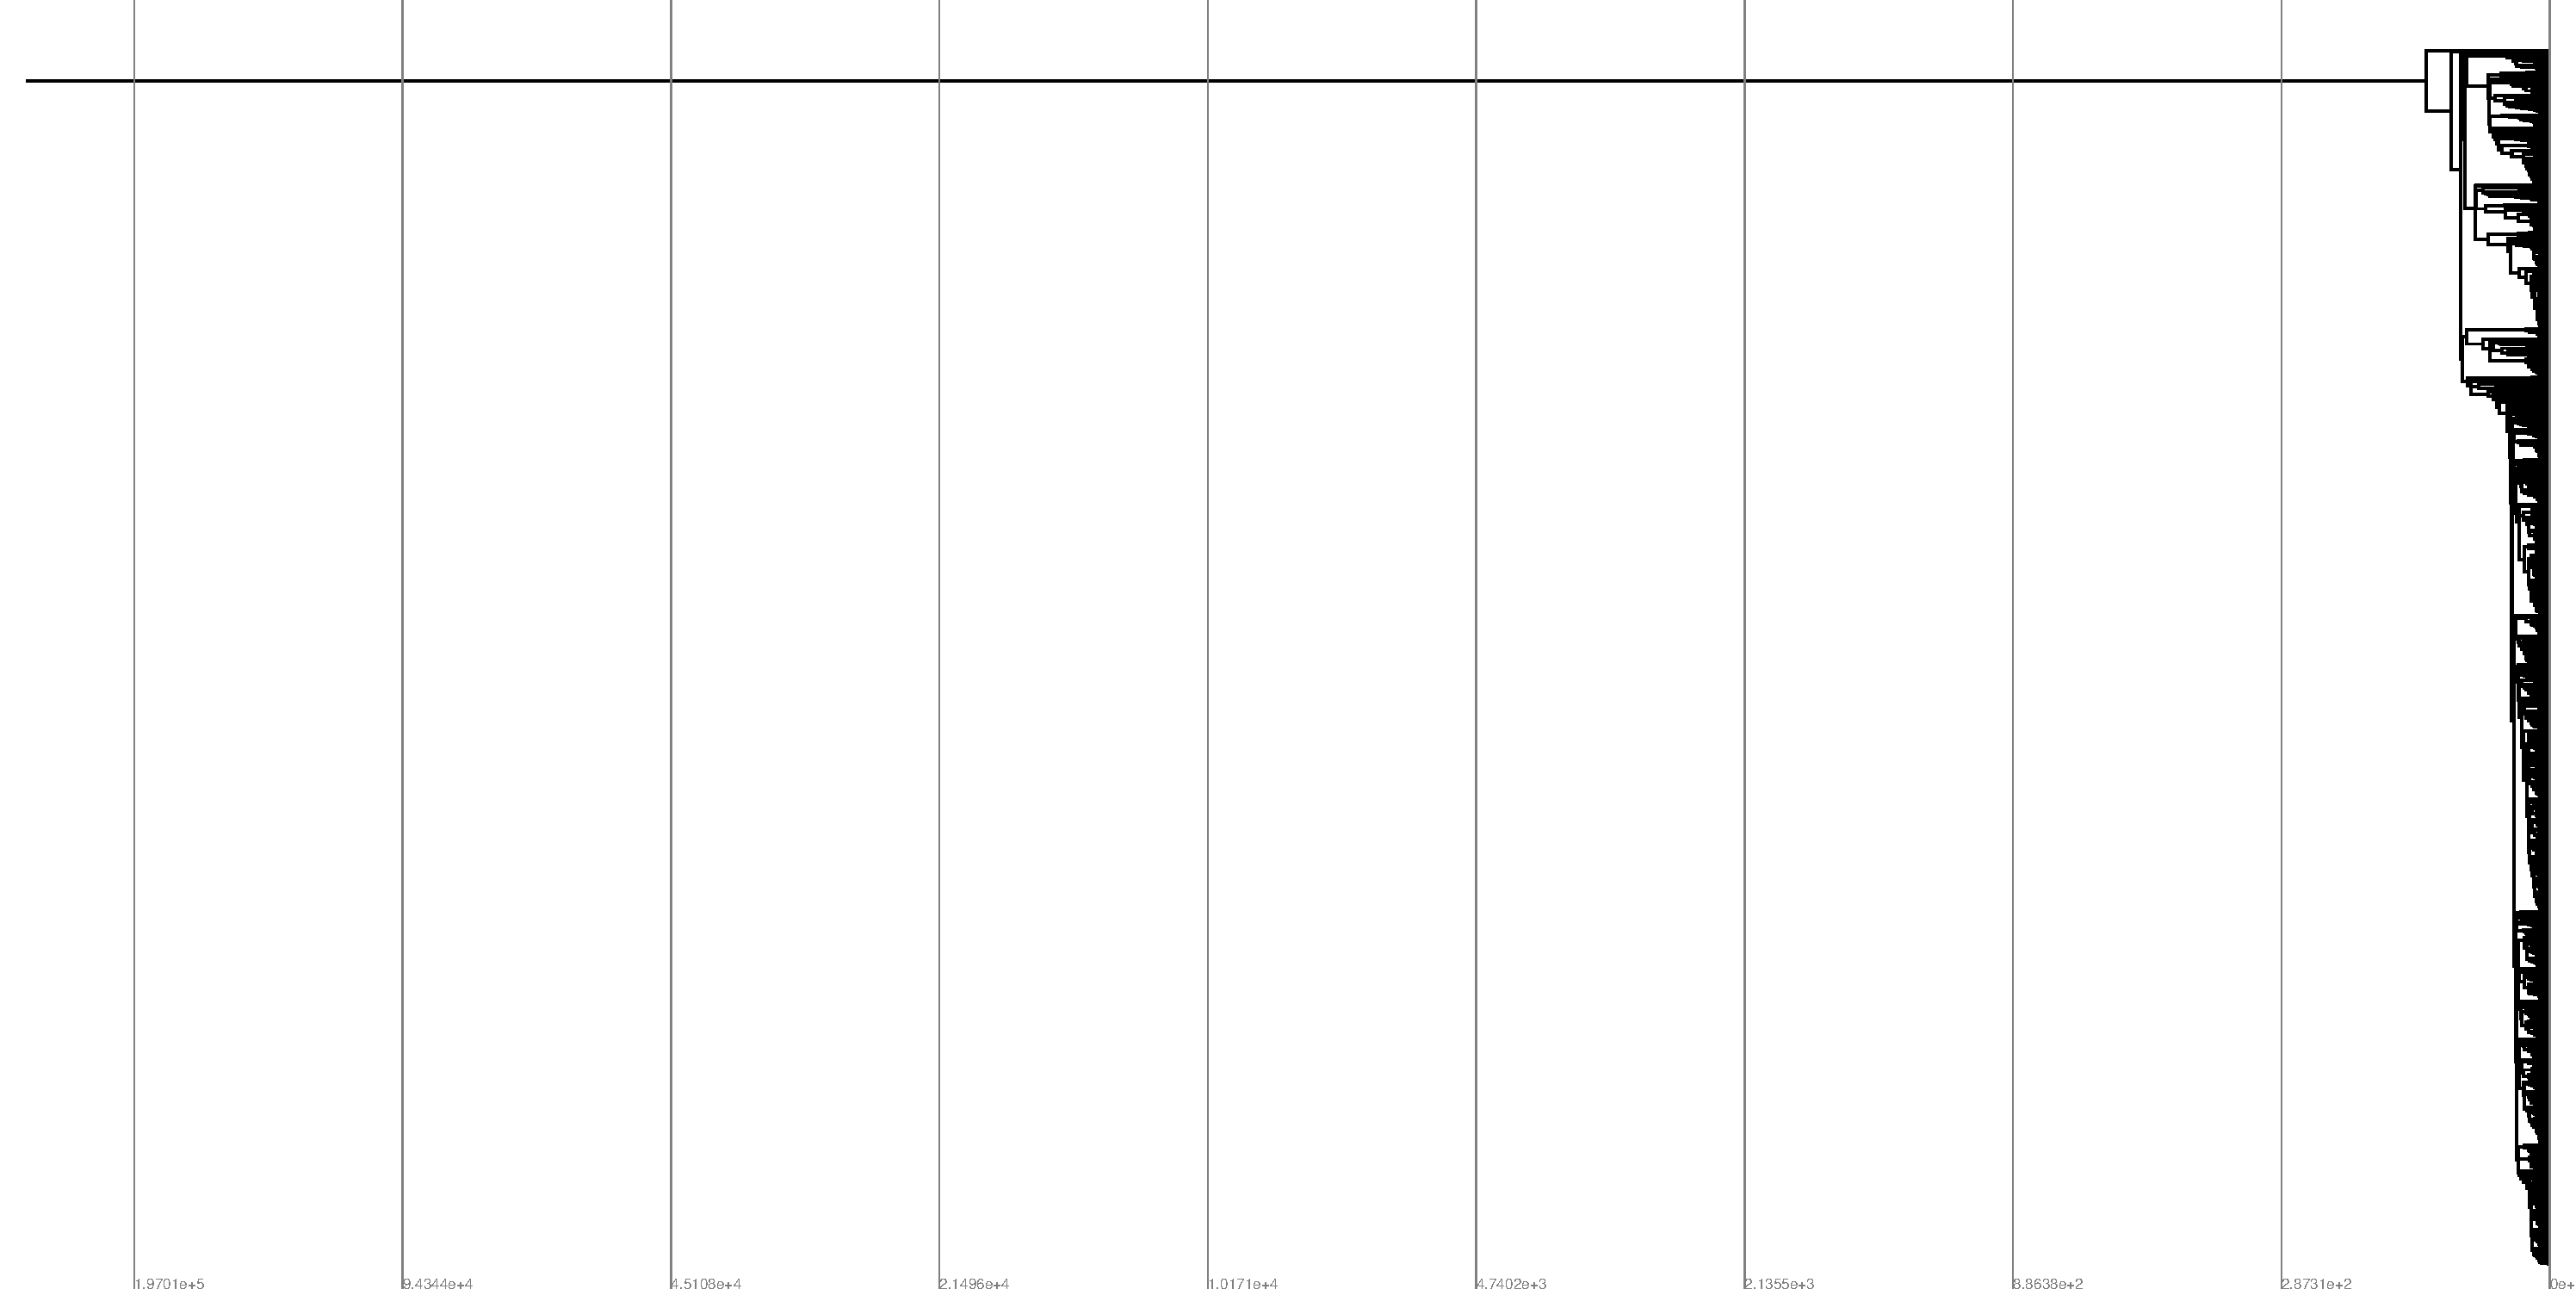
\includegraphics[height=0.12\textheight,width=\textwidth]{img/perfect-tree-phylogenies-log/epoch=7+resolution=3+treatment=8/a=collapsed-phylogeny+epoch=00007+mut_distn=np.random.standard_normal+num_generations=32768+num_islands=1+num_niches=1+p_island_migration=0.01+p_niche_invasion=3.0517578125e-08+population_size=32768+r.../eplicate=0+tournament_size=2+treatment=8+_generation=262144+_index=8+ext=.pdf}
    % \end{noindent}
    \caption{%
      plain}
    % \label{fig:perfect-tree-phylogenies-log:TODO}
  \end{subfigure}

  \caption{%
    Sample reference phylogenies across surveyed evolutionary metrics.
    Each phylogeny has 32,768 leaves.
    Note log-scale $x$ axis.
  }
  \label{fig:perfect-tree-phylogenies-log}
\end{figure*}


Consequently, researchers across many fields have an interest in inferring the processes that shaped a phylogeny by quantifying its topology.
Currently, most research on this topic is either very abstract (e.g., the presence of negative-frequency dependent selection increases phylogenetic diversity) or very specific (e.g., phylogenetic structure can be used to infer cell division rates in solid tumors \citep{lewinsohnStatedependentEvolutionaryModels2023}).
Here, we lay the groundwork for identifying the fingerprints left on phylogenetic structure by a larger range of evolutionary dynamics in a scalable and robust manner.

%Some groundwork has been done in the fields of conservation biology and cancer biology, as well as in artificial life (cite ``tape of life''?) to understand how evolutionary dynamics affect phylogenetic structure (and the fingerprints of evolutionary dynamics on phylogenetic structure) but this is still a rapidly emerging field (be sure to hedge here).
%In particular, existing work has shown x, y and z.

%One major difference between digital study systems and biological study systems is the availability of perfect data.
%In biology, we rely on reconstructions to estimate phylogenetic history; the effect of estimation error on phylometrics is poorly understood.
Historically, digital evolution systems have had the advantage of providing perfectly accurate phylogenetic data, in contrast to the reconstructed phylogenies relied upon in traditional biology.
However, as digital evolution systems scale, issues of data loss and decentralization will make perfect tracking at best inefficient and at worst untenable.
Thus, some systems will likely need to adopt a decentralized, reconstruction-based approach similar to biological data.
%Decentralization will also likely introduce an aspect of spatial structure (i.e., populations will no longer be ``well-mixed'') which will further complicate phylogenetic analyses.
Consequently, if our goal is to use phylogenetic metrics to increase the scalability of our data analysis, we must also understand how robust they are to inaccuracies introduced by reconstruction.
% (maybe briefly cite/mention effect of spatial structure on phylogenies)
Phylogenetic reconstructions in artificial life can be achieved through the recently-developed ``hereditary stratigraphy'' approach, a lightweight annotation scheme that can give tunably-precise information about the phylogenetic history between any two extant organisms.
%In order to put hereditary stratigraphy into practice to better observe digital evolution systems will require an understanding of how ecology and selection pressure manifest in phylogenetic structure and also how potentially confounding factors of estimation uncertainty and spatial structure manifest.
%Indeed, as artificial life systems scale they are becoming more reminsicent of biological systems and these findings will be applicable to phylogenetics work in biology outside of artificial life.

In this paper, we build the following methodological and theoretical foundations that will be needed to use phylogenetic analyses to observe evolutionary dynamics in complex, distributed artificial life systems:
\begin{enumerate}
  \item the ability to perform fast, accurate tree reconstructions for very large distributed populations,
  \item understanding of the relationship between evolutionary dynamics and phylogenetic metrics,
  \item quantification of the effects of reconstruction-induced estimation error on phylogenetic structure, both in terms of the amount of precision required for accuracy and the amount of bias introduced by inadequate precision, and
  \item quantification of the phylogenetic effects of spatial structure, as distributed computation does not support well-mixed populations.
\end{enumerate}

% \begin{enumerate}
% \item how much precision is required for accurate phylogenetic metrics?
% \item if bias is introduced, what type of bias (so could still detect "conservatively")
% \end{enumerate}
